\documentclass{book}
\usepackage[a4paper,top=2.5cm,bottom=2.5cm,left=2.5cm,right=2.5cm]{geometry}
\usepackage{makeidx}
\usepackage{natbib}
\usepackage{graphicx}
\usepackage{multicol}
\usepackage{float}
\usepackage{listings}
\usepackage{color}
\usepackage{ifthen}
\usepackage[table]{xcolor}
\usepackage{textcomp}
\usepackage{alltt}
\usepackage{ifpdf}
\ifpdf
\usepackage[pdftex,
            pagebackref=true,
            colorlinks=true,
            linkcolor=blue,
            unicode
           ]{hyperref}
\else
\usepackage[ps2pdf,
            pagebackref=true,
            colorlinks=true,
            linkcolor=blue,
            unicode
           ]{hyperref}
\usepackage{pspicture}
\fi
\usepackage[utf8]{inputenc}
\usepackage[french]{babel}

\usepackage{mathptmx}
\usepackage[scaled=.90]{helvet}
\usepackage{courier}
\usepackage{sectsty}
\usepackage[titles]{tocloft}
\usepackage{doxygen}
\lstset{language=C++,inputencoding=utf8,basicstyle=\footnotesize,breaklines=true,breakatwhitespace=true,tabsize=8,numbers=left }
\makeindex
\setcounter{tocdepth}{3}
\renewcommand{\footrulewidth}{0.4pt}
\renewcommand{\familydefault}{\sfdefault}
\hfuzz=15pt
\setlength{\emergencystretch}{15pt}
\hbadness=750
\tolerance=750
\begin{document}
\hypersetup{pageanchor=false,citecolor=blue}
\begin{titlepage}
\vspace*{7cm}
\begin{center}
{\Large Calc\-Polo }\\
\vspace*{1cm}
{\large Généré par Doxygen 1.8.1}\\
\vspace*{0.5cm}
{\small Dimanche Juin 17 2012 17:26:14}\\
\end{center}
\end{titlepage}
\clearemptydoublepage
\pagenumbering{roman}
\tableofcontents
\clearemptydoublepage
\pagenumbering{arabic}
\hypersetup{pageanchor=true,citecolor=blue}
\chapter{Index des classes}
\section{Hiérarchie des classes}
Cette liste d'héritage est classée approximativement par ordre alphabétique \-:\begin{DoxyCompactList}
\item \contentsline{section}{Collection\-Pile}{\pageref{class_collection_pile}}{}
\item \contentsline{section}{Dom}{\pageref{class_dom}}{}
\item \contentsline{section}{Donnee}{\pageref{class_donnee}}{}
\begin{DoxyCompactList}
\item \contentsline{section}{D}{\pageref{class_d}}{}
\begin{DoxyCompactList}
\item \contentsline{section}{Complexe}{\pageref{class_complexe}}{}
\item \contentsline{section}{Constante}{\pageref{class_constante}}{}
\begin{DoxyCompactList}
\item \contentsline{section}{Entier}{\pageref{class_entier}}{}
\item \contentsline{section}{Rationnel}{\pageref{class_rationnel}}{}
\item \contentsline{section}{Reel}{\pageref{class_reel}}{}
\end{DoxyCompactList}
\end{DoxyCompactList}
\item \contentsline{section}{Expression}{\pageref{class_expression}}{}
\end{DoxyCompactList}
\item \contentsline{section}{Donnee\-Exception}{\pageref{class_donnee_exception}}{}
\item \contentsline{section}{Donnee\-Factory}{\pageref{class_donnee_factory}}{}
\item \contentsline{section}{Main\-Window}{\pageref{class_main_window}}{}
\item \contentsline{section}{Memento}{\pageref{class_memento}}{}
\item \contentsline{section}{Pile}{\pageref{class_pile}}{}
\end{DoxyCompactList}

\chapter{Index des classes}
\section{Liste des classes}
Liste des classes, structures, unions et interfaces avec une brève description \-:\begin{DoxyCompactList}
\item\contentsline{section}{\hyperlink{class_collection_pile}{Collection\-Pile} }{\pageref{class_collection_pile}}{}
\item\contentsline{section}{\hyperlink{class_complexe}{Complexe} }{\pageref{class_complexe}}{}
\item\contentsline{section}{\hyperlink{class_constante}{Constante} }{\pageref{class_constante}}{}
\item\contentsline{section}{\hyperlink{class_d}{D} }{\pageref{class_d}}{}
\item\contentsline{section}{\hyperlink{class_dom}{Dom} }{\pageref{class_dom}}{}
\item\contentsline{section}{\hyperlink{class_donnee}{Donnee} }{\pageref{class_donnee}}{}
\item\contentsline{section}{\hyperlink{class_donnee_exception}{Donnee\-Exception} }{\pageref{class_donnee_exception}}{}
\item\contentsline{section}{\hyperlink{class_donnee_factory}{Donnee\-Factory} }{\pageref{class_donnee_factory}}{}
\item\contentsline{section}{\hyperlink{class_entier}{Entier} }{\pageref{class_entier}}{}
\item\contentsline{section}{\hyperlink{class_expression}{Expression} }{\pageref{class_expression}}{}
\item\contentsline{section}{\hyperlink{class_main_window}{Main\-Window} }{\pageref{class_main_window}}{}
\item\contentsline{section}{\hyperlink{class_memento}{Memento} }{\pageref{class_memento}}{}
\item\contentsline{section}{\hyperlink{class_pile}{Pile} }{\pageref{class_pile}}{}
\item\contentsline{section}{\hyperlink{class_rationnel}{Rationnel} }{\pageref{class_rationnel}}{}
\item\contentsline{section}{\hyperlink{class_reel}{Reel} }{\pageref{class_reel}}{}
\end{DoxyCompactList}

\chapter{Index des fichiers}
\section{Liste des fichiers}
Liste de tous les fichiers documentés avec une brève description \-:\begin{DoxyCompactList}
\item\contentsline{section}{\hyperlink{_collection_pile_8h}{Collection\-Pile.\-h} \\*\hyperlink{class_collection_pile}{Collection\-Pile} contient la classe \hyperlink{class_collection_pile}{Collection\-Pile} qui herite de vector et contient les piles pour ctrl + Z/ctrl + Y (undo/redo) }{\pageref{_collection_pile_8h}}{}
\item\contentsline{section}{\hyperlink{_complexe_8h}{Complexe.\-h} \\*\hyperlink{class_complexe}{Complexe} contient la classe complexe qui h�rite de \hyperlink{class_d}{D}, elle m�me h�ritant de Donn�e. cette classe sert � cr�er les objets complexes a\&b (lorsque le mode complexe est activ�) }{\pageref{_complexe_8h}}{}
\item\contentsline{section}{\hyperlink{_constante_8h}{Constante.\-h} \\*\hyperlink{class_constante}{Constante} Class abstraite h�ritant de \hyperlink{class_d}{D} (qui h�rite de Donn�e) et engeandrant les classe \hyperlink{class_reel}{Reel}, \hyperlink{class_rationnel}{Rationnel}, \hyperlink{class_entier}{Entier} }{\pageref{_constante_8h}}{}
\item\contentsline{section}{\hyperlink{_d_8h}{D.\-h} \\*\hyperlink{class_d}{D} Classe h�ritant de \hyperlink{class_donnee}{Donnee} et engeandrant \hyperlink{class_complexe}{Complexe} }{\pageref{_d_8h}}{}
\item\contentsline{section}{\hyperlink{_dom_8h}{Dom.\-h} \\*\hyperlink{class_dom}{Dom} classe contenant les m�thodes d'�criture et de lecture de piles }{\pageref{_dom_8h}}{}
\item\contentsline{section}{\hyperlink{_donnee_8h}{Donnee.\-h} \\*Donne contient la classe abstraite qui chapeaute les classes des diff�rents types de donn�es }{\pageref{_donnee_8h}}{}
\item\contentsline{section}{\hyperlink{_donnee_exception_8h}{Donnee\-Exception.\-h} \\*Donne\-Exception classe qui g�re les exceptions }{\pageref{_donnee_exception_8h}}{}
\item\contentsline{section}{\hyperlink{_donnee_factory_8h}{Donnee\-Factory.\-h} \\*Donne\-Factory Classe � instance unique qui cr�er les Objets de type \hyperlink{class_donnee}{Donnee} (\hyperlink{class_reel}{Reel}, \hyperlink{class_rationnel}{Rationnel}, \hyperlink{class_entier}{Entier}, \hyperlink{class_complexe}{Complexe}) }{\pageref{_donnee_factory_8h}}{}
\item\contentsline{section}{\hyperlink{_entier_8h}{Entier.\-h} \\*\hyperlink{class_entier}{Entier} contient la classe permet de g�n�rer les objets stockant les entiers }{\pageref{_entier_8h}}{}
\item\contentsline{section}{\hyperlink{_expression_8h}{Expression.\-h} \\*\hyperlink{class_expression}{Expression} contient la classe permet de g�n�rer les objets stockant les expressions }{\pageref{_expression_8h}}{}
\item\contentsline{section}{\hyperlink{_main_window_8h}{Main\-Window.\-h} \\*\hyperlink{class_main_window}{Main\-Window} Classe de l'affichage de la fen�tre principale }{\pageref{_main_window_8h}}{}
\item\contentsline{section}{\hyperlink{_memento_8h}{Memento.\-h} \\*\hyperlink{class_memento}{Memento} Comprend les m�thodes n�cessaire � la r�alisation de undo/redo }{\pageref{_memento_8h}}{}
\item\contentsline{section}{\hyperlink{_pile_8h}{Pile.\-h} \\*\hyperlink{class_pile}{Pile} Classe de nos piles, h�ritant de Q\-Stack. Ce sont des piles de \hyperlink{class_donnee}{Donnee} }{\pageref{_pile_8h}}{}
\item\contentsline{section}{\hyperlink{_rationnel_8h}{Rationnel.\-h} \\*\hyperlink{class_rationnel}{Rationnel} contient la classe permet de g�n�rer les objets stockant les rationnels }{\pageref{_rationnel_8h}}{}
\item\contentsline{section}{\hyperlink{_reel_8h}{Reel.\-h} \\*\hyperlink{class_reel}{Reel} contient la classe permet de g�n�rer les objets stockant les r�els }{\pageref{_reel_8h}}{}
\end{DoxyCompactList}

\chapter{Documentation des classes}
\hypertarget{class_collection_pile}{\section{Référence de la classe Collection\-Pile}
\label{class_collection_pile}\index{Collection\-Pile@{Collection\-Pile}}
}
\subsection*{Fonctions membres publiques}
\begin{DoxyCompactItemize}
\item 
\hypertarget{class_collection_pile_ab6c67317876c4b74548d5459d61bfaff}{void {\bfseries add\-Pile} (\hyperlink{class_pile}{Pile} $\ast$p)}\label{class_collection_pile_ab6c67317876c4b74548d5459d61bfaff}

\item 
\hypertarget{class_collection_pile_a6685a7063ffe1a8951aed57042f8fe31}{void {\bfseries set\-Actif} (int a)}\label{class_collection_pile_a6685a7063ffe1a8951aed57042f8fe31}

\item 
\hypertarget{class_collection_pile_a265a8d02d0c37f99ca0d2df20fcc2b3f}{int {\bfseries get\-Actif} ()}\label{class_collection_pile_a265a8d02d0c37f99ca0d2df20fcc2b3f}

\end{DoxyCompactItemize}
\subsection*{Fonctions membres publiques statiques}
\begin{DoxyCompactItemize}
\item 
\hypertarget{class_collection_pile_af542ecfe521b494bb9596f586784ee3a}{static \hyperlink{class_collection_pile}{Collection\-Pile} \& {\bfseries get\-Instance} ()}\label{class_collection_pile_af542ecfe521b494bb9596f586784ee3a}

\item 
\hypertarget{class_collection_pile_a4dec5876d1013bd2163fa579b5558285}{static void {\bfseries release\-Instance} ()}\label{class_collection_pile_a4dec5876d1013bd2163fa579b5558285}

\end{DoxyCompactItemize}


\subsection{Description détaillée}

\begin{DoxyParams}{Paramètres}
{\em instance} & l'instance unique de notre Collection \\
\hline
{\em actif} & rang de la pile active \\
\hline
\end{DoxyParams}


La documentation de cette classe a été générée à partir des fichiers suivants \-:\begin{DoxyCompactItemize}
\item 
\hyperlink{_collection_pile_8h}{Collection\-Pile.\-h}\item 
Collection\-Pile.\-cpp\end{DoxyCompactItemize}

\hypertarget{class_complexe}{\section{Référence de la classe Complexe}
\label{class_complexe}\index{Complexe@{Complexe}}
}
Graphe d'héritage de Complexe\-:\begin{figure}[H]
\begin{center}
\leavevmode
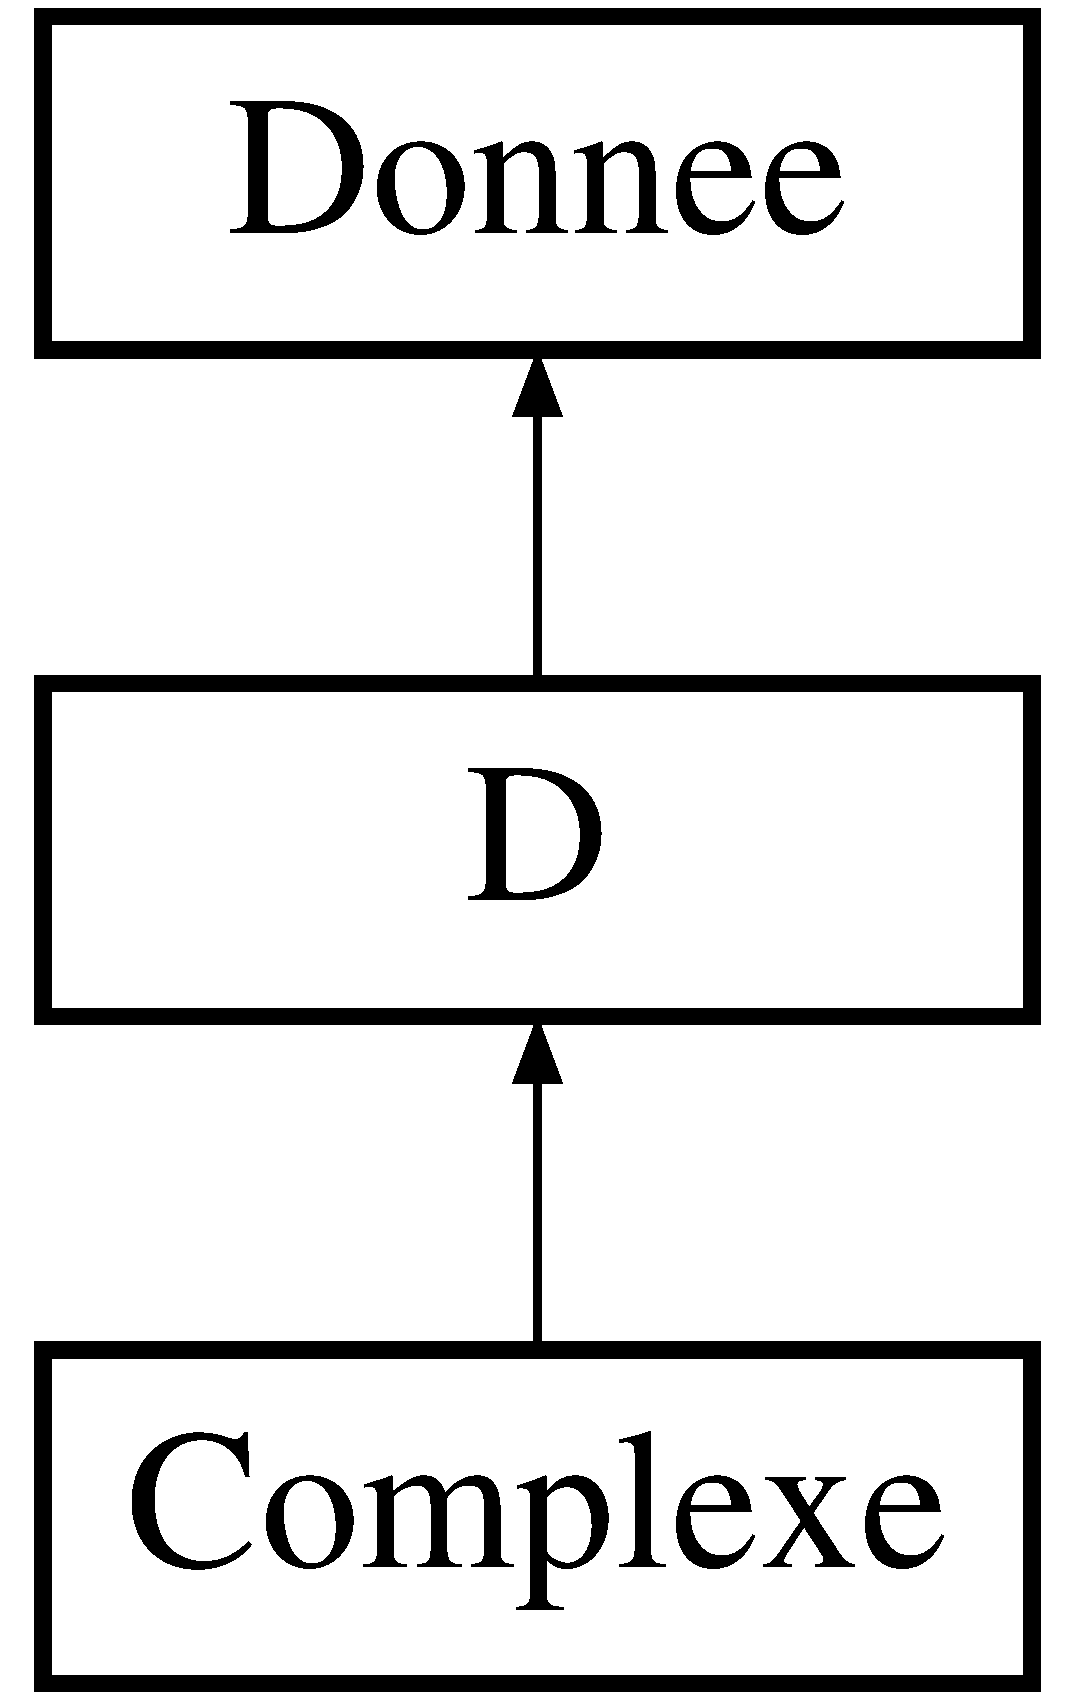
\includegraphics[height=3.000000cm]{class_complexe}
\end{center}
\end{figure}
\subsection*{Fonctions membres publiques}
\begin{DoxyCompactItemize}
\item 
\hypertarget{class_complexe_a2465faa5cc94a91a261f0f7720c1553f}{{\bfseries Complexe} (\hyperlink{class_constante}{Constante} $\ast$\-\_\-re=0, \hyperlink{class_constante}{Constante} $\ast$\-\_\-im=0)}\label{class_complexe_a2465faa5cc94a91a261f0f7720c1553f}

\item 
\hypertarget{class_complexe_a8290a8acf5c2eea42f033da20924192a}{\hyperlink{class_donnee}{Donnee} $\ast$ {\bfseries conjugue} ()}\label{class_complexe_a8290a8acf5c2eea42f033da20924192a}

\item 
\hypertarget{class_complexe_a8ae4f6c56823f3dd6522883b3dbcf059}{{\bfseries Complexe} (const Q\-String \&s)}\label{class_complexe_a8ae4f6c56823f3dd6522883b3dbcf059}

\item 
\hypertarget{class_complexe_a1941d1f57fa3e45ebb2a7391e8d528e1}{\hyperlink{class_donnee}{Donnee} $\ast$ {\bfseries operator+} (\hyperlink{class_donnee}{Donnee} \&t)}\label{class_complexe_a1941d1f57fa3e45ebb2a7391e8d528e1}

\item 
\hypertarget{class_complexe_ae1f5eaa6bd60b539c8191399ffa5658d}{\hyperlink{class_donnee}{Donnee} $\ast$ {\bfseries operator/} (\hyperlink{class_donnee}{Donnee} \&t)}\label{class_complexe_ae1f5eaa6bd60b539c8191399ffa5658d}

\item 
\hypertarget{class_complexe_a7a36cc4cc516e0e4828e0e6fb16ba23c}{\hyperlink{class_donnee}{Donnee} $\ast$ {\bfseries operator$\ast$} (\hyperlink{class_donnee}{Donnee} \&t)}\label{class_complexe_a7a36cc4cc516e0e4828e0e6fb16ba23c}

\item 
\hypertarget{class_complexe_a3ff42a9947cc747c742cc2e5fcd2dab5}{\hyperlink{class_donnee}{Donnee} $\ast$ {\bfseries operator-\/} (\hyperlink{class_donnee}{Donnee} \&t)}\label{class_complexe_a3ff42a9947cc747c742cc2e5fcd2dab5}

\item 
\hypertarget{class_complexe_a0039f536b7a0e339beec2f0135573237}{\hyperlink{class_donnee}{Donnee} $\ast$ {\bfseries sign} ()}\label{class_complexe_a0039f536b7a0e339beec2f0135573237}

\item 
\hypertarget{class_complexe_a5092fb9333bba54eadb4666c17ede45f}{\hyperlink{class_constante}{Constante} $\ast$ {\bfseries get\-Re} ()}\label{class_complexe_a5092fb9333bba54eadb4666c17ede45f}

\item 
\hypertarget{class_complexe_a06a17e03b95c2360cb38831e8766fe7d}{\hyperlink{class_constante}{Constante} $\ast$ {\bfseries get\-Im} ()}\label{class_complexe_a06a17e03b95c2360cb38831e8766fe7d}

\item 
\hypertarget{class_complexe_a965e1607226c63c751a33b8529bb294d}{Q\-String {\bfseries to\-Q\-String} ()}\label{class_complexe_a965e1607226c63c751a33b8529bb294d}

\end{DoxyCompactItemize}


La documentation de cette classe a été générée à partir des fichiers suivants \-:\begin{DoxyCompactItemize}
\item 
\hyperlink{_complexe_8h}{Complexe.\-h}\item 
complexe.\-cpp\end{DoxyCompactItemize}

\hypertarget{class_constante}{\section{Référence de la classe Constante}
\label{class_constante}\index{Constante@{Constante}}
}
Graphe d'héritage de Constante\-:\begin{figure}[H]
\begin{center}
\leavevmode
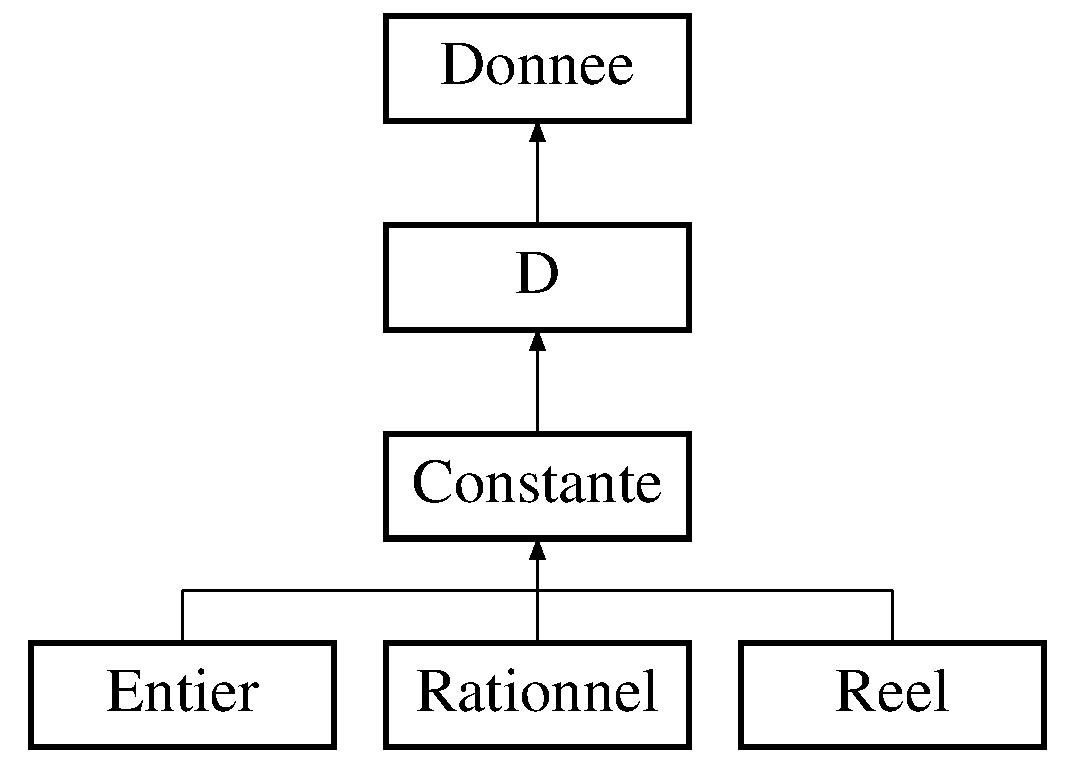
\includegraphics[height=4.000000cm]{class_constante}
\end{center}
\end{figure}
\subsection*{Fonctions membres publiques}
\begin{DoxyCompactItemize}
\item 
\hypertarget{class_constante_a914d72396ac8ee3c9a59fd6d4817feb4}{virtual \hyperlink{class_donnee}{Donnee} $\ast$ {\bfseries operator+} (\hyperlink{class_donnee}{Donnee} \&t)=0}\label{class_constante_a914d72396ac8ee3c9a59fd6d4817feb4}

\item 
\hypertarget{class_constante_ac4772c2a34869f1da07f174cc3331ae3}{virtual \hyperlink{class_donnee}{Donnee} $\ast$ {\bfseries operator/} (\hyperlink{class_donnee}{Donnee} \&t)=0}\label{class_constante_ac4772c2a34869f1da07f174cc3331ae3}

\item 
\hypertarget{class_constante_a0b06eab8cf8a92715348476b74b30f84}{virtual \hyperlink{class_donnee}{Donnee} $\ast$ {\bfseries operator$\ast$} (\hyperlink{class_donnee}{Donnee} \&t)=0}\label{class_constante_a0b06eab8cf8a92715348476b74b30f84}

\item 
\hypertarget{class_constante_a5ecc23da0dc7eb89e02896a22029f222}{virtual \hyperlink{class_donnee}{Donnee} $\ast$ {\bfseries operator-\/} (\hyperlink{class_donnee}{Donnee} \&t)=0}\label{class_constante_a5ecc23da0dc7eb89e02896a22029f222}

\item 
\hypertarget{class_constante_a6f94123b249adbb3f839688b1fa90908}{virtual \hyperlink{class_donnee}{Donnee} $\ast$ {\bfseries pow} (\hyperlink{class_donnee}{Donnee} \&t)=0}\label{class_constante_a6f94123b249adbb3f839688b1fa90908}

\item 
\hypertarget{class_constante_a77547d8149c75a147c20a575463861b4}{virtual \hyperlink{class_donnee}{Donnee} $\ast$ {\bfseries sign} ()=0}\label{class_constante_a77547d8149c75a147c20a575463861b4}

\item 
\hypertarget{class_constante_ae9114c2384356454a895bdc9be526fd1}{virtual \hyperlink{class_donnee}{Donnee} $\ast$ {\bfseries sinus} (bool degre)=0}\label{class_constante_ae9114c2384356454a895bdc9be526fd1}

\item 
\hypertarget{class_constante_a68bbf0a45b4df44285e6061e9ece41cb}{virtual \hyperlink{class_donnee}{Donnee} $\ast$ {\bfseries cosinus} (bool degre)=0}\label{class_constante_a68bbf0a45b4df44285e6061e9ece41cb}

\item 
\hypertarget{class_constante_a586760fc3789d45d2fc22c63d5ac0679}{virtual \hyperlink{class_donnee}{Donnee} $\ast$ {\bfseries tangente} (bool degre)=0}\label{class_constante_a586760fc3789d45d2fc22c63d5ac0679}

\item 
\hypertarget{class_constante_a630282a8ee4ff579615eecf06c2bff81}{virtual \hyperlink{class_donnee}{Donnee} $\ast$ {\bfseries sinush} (bool degre)=0}\label{class_constante_a630282a8ee4ff579615eecf06c2bff81}

\item 
\hypertarget{class_constante_af447d1a704ccd3855741328c4ff97300}{virtual \hyperlink{class_donnee}{Donnee} $\ast$ {\bfseries cosinush} (bool degre)=0}\label{class_constante_af447d1a704ccd3855741328c4ff97300}

\item 
\hypertarget{class_constante_a32e1d620c11e78b8318383924a5e9774}{virtual \hyperlink{class_donnee}{Donnee} $\ast$ {\bfseries tangenteh} (bool degre)=0}\label{class_constante_a32e1d620c11e78b8318383924a5e9774}

\item 
\hypertarget{class_constante_a63658ad4998f3b122b9f4f9f02a4f525}{virtual \hyperlink{class_donnee}{Donnee} $\ast$ {\bfseries ln} ()=0}\label{class_constante_a63658ad4998f3b122b9f4f9f02a4f525}

\item 
\hypertarget{class_constante_a6d96efcf73d825f28c9d3d155ecc983a}{virtual \hyperlink{class_donnee}{Donnee} $\ast$ {\bfseries log} ()=0}\label{class_constante_a6d96efcf73d825f28c9d3d155ecc983a}

\item 
\hypertarget{class_constante_ae7a6e1a008b871e48dca3923baa5514e}{virtual \hyperlink{class_donnee}{Donnee} $\ast$ {\bfseries inv} ()=0}\label{class_constante_ae7a6e1a008b871e48dca3923baa5514e}

\item 
\hypertarget{class_constante_a3e057173655eabe182ed4b8c09ad2ab0}{virtual \hyperlink{class_donnee}{Donnee} $\ast$ {\bfseries sqrt} ()=0}\label{class_constante_a3e057173655eabe182ed4b8c09ad2ab0}

\item 
\hypertarget{class_constante_ae106a1a6e582a5779a1dac6c0fc037b4}{virtual \hyperlink{class_donnee}{Donnee} $\ast$ {\bfseries sqr} ()=0}\label{class_constante_ae106a1a6e582a5779a1dac6c0fc037b4}

\item 
\hypertarget{class_constante_ac0df5e4a4d4116c36cd252abaaf9de3a}{virtual \hyperlink{class_donnee}{Donnee} $\ast$ {\bfseries cube} ()=0}\label{class_constante_ac0df5e4a4d4116c36cd252abaaf9de3a}

\item 
\hypertarget{class_constante_a6ead49eb4298a95ed7c90012e1b272ff}{virtual Q\-String {\bfseries eval} ()}\label{class_constante_a6ead49eb4298a95ed7c90012e1b272ff}

\end{DoxyCompactItemize}


La documentation de cette classe a été générée à partir du fichier suivant \-:\begin{DoxyCompactItemize}
\item 
\hyperlink{_constante_8h}{Constante.\-h}\end{DoxyCompactItemize}

\hypertarget{class_d}{\section{Référence de la classe D}
\label{class_d}\index{D@{D}}
}
Graphe d'héritage de D\-:\begin{figure}[H]
\begin{center}
\leavevmode
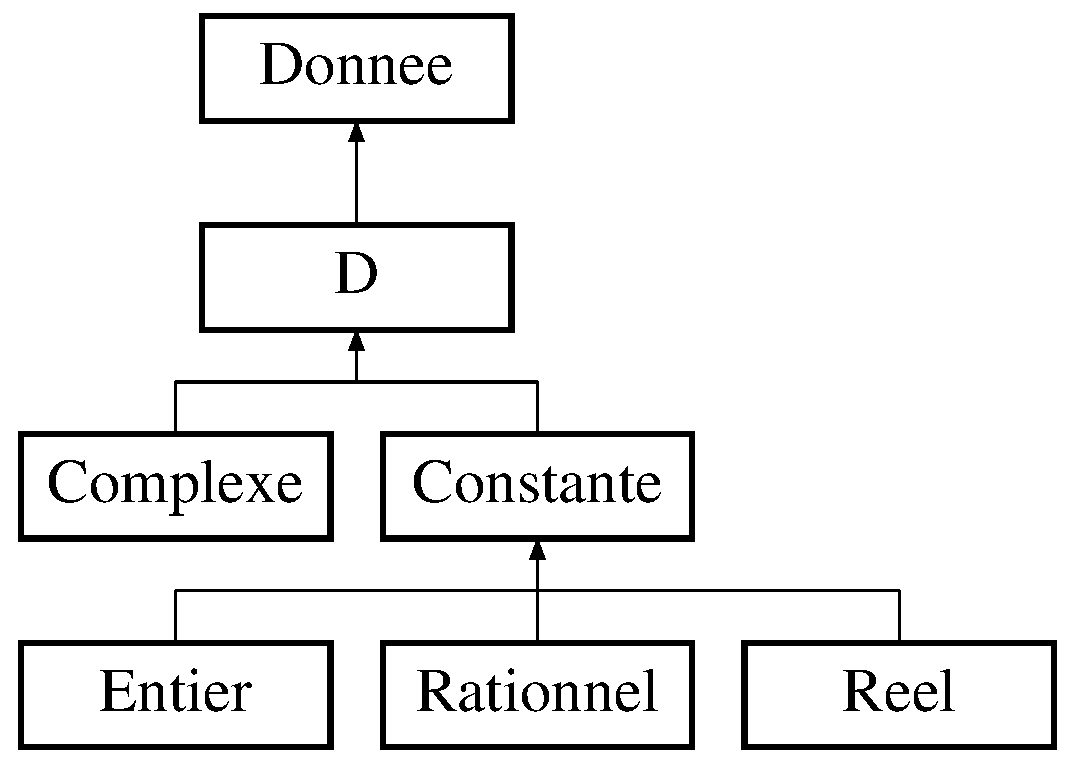
\includegraphics[height=4.000000cm]{class_d}
\end{center}
\end{figure}
\subsection*{Additional Inherited Members}


La documentation de cette classe a été générée à partir du fichier suivant \-:\begin{DoxyCompactItemize}
\item 
\hyperlink{_d_8h}{D.\-h}\end{DoxyCompactItemize}

\hypertarget{class_dom}{\section{Référence de la classe Dom}
\label{class_dom}\index{Dom@{Dom}}
}
\subsection*{Fonctions membres publiques}
\begin{DoxyCompactItemize}
\item 
\hypertarget{class_dom_a76622d9817909851b9e7ba8a9b3d2614}{{\bfseries Dom} (\hyperlink{class_pile}{Pile} \&p)}\label{class_dom_a76622d9817909851b9e7ba8a9b3d2614}

\item 
\hypertarget{class_dom_a76e1a406daef8ed0e1bea3733575eb7f}{void {\bfseries ecrire} (Q\-String file\-Name)}\label{class_dom_a76e1a406daef8ed0e1bea3733575eb7f}

\item 
\hypertarget{class_dom_a0134557ad01388c484bb1661e1962ce1}{void {\bfseries lire} (Q\-String file\-Name)}\label{class_dom_a0134557ad01388c484bb1661e1962ce1}

\end{DoxyCompactItemize}


La documentation de cette classe a été générée à partir des fichiers suivants \-:\begin{DoxyCompactItemize}
\item 
\hyperlink{_dom_8h}{Dom.\-h}\item 
dom.\-cpp\end{DoxyCompactItemize}

\hypertarget{class_donnee}{\section{Référence de la classe Donnee}
\label{class_donnee}\index{Donnee@{Donnee}}
}
Graphe d'héritage de Donnee\-:\begin{figure}[H]
\begin{center}
\leavevmode
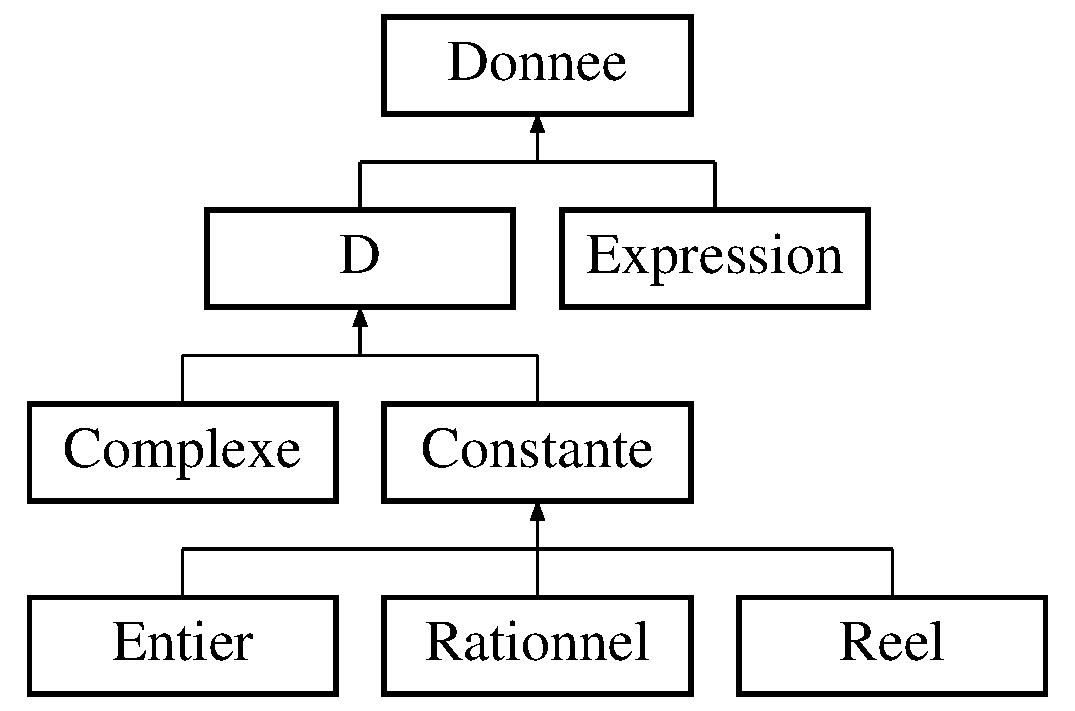
\includegraphics[height=4.000000cm]{class_donnee}
\end{center}
\end{figure}
\subsection*{Fonctions membres publiques}
\begin{DoxyCompactItemize}
\item 
\hypertarget{class_donnee_ad5d08758184849a5b935c897eb950c61}{virtual \hyperlink{class_donnee}{Donnee} $\ast$ {\bfseries operator+} (\hyperlink{class_donnee}{Donnee} \&t)=0}\label{class_donnee_ad5d08758184849a5b935c897eb950c61}

\item 
\hypertarget{class_donnee_ad87f5946973ae658c3f182074fe88c5c}{virtual \hyperlink{class_donnee}{Donnee} $\ast$ {\bfseries operator/} (\hyperlink{class_donnee}{Donnee} \&t)=0}\label{class_donnee_ad87f5946973ae658c3f182074fe88c5c}

\item 
\hypertarget{class_donnee_a3af8060fd9f5523dd06b9024dbf195fd}{virtual \hyperlink{class_donnee}{Donnee} $\ast$ {\bfseries operator$\ast$} (\hyperlink{class_donnee}{Donnee} \&t)=0}\label{class_donnee_a3af8060fd9f5523dd06b9024dbf195fd}

\item 
\hypertarget{class_donnee_ab6d0c4a0e70f03aa17cab93d947574a5}{virtual \hyperlink{class_donnee}{Donnee} $\ast$ {\bfseries operator-\/} (\hyperlink{class_donnee}{Donnee} \&t)=0}\label{class_donnee_ab6d0c4a0e70f03aa17cab93d947574a5}

\item 
\hypertarget{class_donnee_a9637072de31f20b86ca551ac6285487b}{virtual \hyperlink{class_donnee}{Donnee} $\ast$ {\bfseries pow} (\hyperlink{class_donnee}{Donnee} \&t)}\label{class_donnee_a9637072de31f20b86ca551ac6285487b}

\item 
\hypertarget{class_donnee_a7195768b00b91ec0c59c7b958e688a76}{virtual \hyperlink{class_donnee}{Donnee} $\ast$ {\bfseries mod} (\hyperlink{class_donnee}{Donnee} \&t)}\label{class_donnee_a7195768b00b91ec0c59c7b958e688a76}

\item 
\hypertarget{class_donnee_a8376bc550884afe8707bfd0b96566c9a}{virtual \hyperlink{class_donnee}{Donnee} $\ast$ {\bfseries sign} ()}\label{class_donnee_a8376bc550884afe8707bfd0b96566c9a}

\item 
\hypertarget{class_donnee_ac451ff3716c39aab474758ef60842efd}{virtual \hyperlink{class_donnee}{Donnee} $\ast$ {\bfseries sinus} (bool degre=false)}\label{class_donnee_ac451ff3716c39aab474758ef60842efd}

\item 
\hypertarget{class_donnee_a7acf23e9df7b283ee250979c45ffd552}{virtual \hyperlink{class_donnee}{Donnee} $\ast$ {\bfseries cosinus} (bool degre=false)}\label{class_donnee_a7acf23e9df7b283ee250979c45ffd552}

\item 
\hypertarget{class_donnee_ac33001ccfe52e44ddfcb2867b3237071}{virtual \hyperlink{class_donnee}{Donnee} $\ast$ {\bfseries tangente} (bool degre=false)}\label{class_donnee_ac33001ccfe52e44ddfcb2867b3237071}

\item 
\hypertarget{class_donnee_adf2596df9d32c19e4e11f14e427463a3}{virtual \hyperlink{class_donnee}{Donnee} $\ast$ {\bfseries sinush} (bool degre=false)}\label{class_donnee_adf2596df9d32c19e4e11f14e427463a3}

\item 
\hypertarget{class_donnee_aaf9c1fff535f07bbccacf9a84bf93c0f}{virtual \hyperlink{class_donnee}{Donnee} $\ast$ {\bfseries cosinush} (bool degre=false)}\label{class_donnee_aaf9c1fff535f07bbccacf9a84bf93c0f}

\item 
\hypertarget{class_donnee_a7e9b76d263322a608be941806141253f}{virtual \hyperlink{class_donnee}{Donnee} $\ast$ {\bfseries tangenteh} (bool degre=false)}\label{class_donnee_a7e9b76d263322a608be941806141253f}

\item 
\hypertarget{class_donnee_ae9d27263f4b2ef0db3cafe2c2dc5cb91}{virtual \hyperlink{class_donnee}{Donnee} $\ast$ {\bfseries ln} ()}\label{class_donnee_ae9d27263f4b2ef0db3cafe2c2dc5cb91}

\item 
\hypertarget{class_donnee_a9240a3498980483358186327a7f214f8}{virtual \hyperlink{class_donnee}{Donnee} $\ast$ {\bfseries log} ()}\label{class_donnee_a9240a3498980483358186327a7f214f8}

\item 
\hypertarget{class_donnee_a4d8949660f58c2a7504489773edc985c}{virtual \hyperlink{class_donnee}{Donnee} $\ast$ {\bfseries inv} ()}\label{class_donnee_a4d8949660f58c2a7504489773edc985c}

\item 
\hypertarget{class_donnee_a03b474f5f379b4b99c7c42aaa2d5eecd}{virtual \hyperlink{class_donnee}{Donnee} $\ast$ {\bfseries sqrt} ()}\label{class_donnee_a03b474f5f379b4b99c7c42aaa2d5eecd}

\item 
\hypertarget{class_donnee_a116e1c4326d5c6b938f90c9ad4ae26c3}{virtual \hyperlink{class_donnee}{Donnee} $\ast$ {\bfseries sqr} ()}\label{class_donnee_a116e1c4326d5c6b938f90c9ad4ae26c3}

\item 
\hypertarget{class_donnee_a40a46fbde2cfe5df2a92661e94bf8b3b}{virtual \hyperlink{class_donnee}{Donnee} $\ast$ {\bfseries cube} ()}\label{class_donnee_a40a46fbde2cfe5df2a92661e94bf8b3b}

\item 
\hypertarget{class_donnee_ac12cf380eacf2a022ec966f879172ebd}{virtual \hyperlink{class_donnee}{Donnee} $\ast$ {\bfseries fact} ()}\label{class_donnee_ac12cf380eacf2a022ec966f879172ebd}

\item 
\hypertarget{class_donnee_a0c5db4e00d821a7ec411e98a9d15730b}{virtual Q\-String {\bfseries eval} ()}\label{class_donnee_a0c5db4e00d821a7ec411e98a9d15730b}

\item 
\hypertarget{class_donnee_a92bcbd4d69bdbc30cc3379c4ffbcb760}{virtual Q\-String {\bfseries to\-Q\-String} ()=0}\label{class_donnee_a92bcbd4d69bdbc30cc3379c4ffbcb760}

\end{DoxyCompactItemize}
\subsection*{Fonctions membres publiques statiques}
\begin{DoxyCompactItemize}
\item 
\hypertarget{class_donnee_ab195ba9c738ca7a68e46619c05efc25d}{static bool {\bfseries is\-Entier} (const Q\-String \&s)}\label{class_donnee_ab195ba9c738ca7a68e46619c05efc25d}

\item 
\hypertarget{class_donnee_a3bf8894c20219f055032e5811606e248}{static bool {\bfseries is\-Reel} (const Q\-String \&s)}\label{class_donnee_a3bf8894c20219f055032e5811606e248}

\item 
\hypertarget{class_donnee_af485090a75b51f1784d60e55a1eefd1a}{static bool {\bfseries is\-Rationnel} (const Q\-String \&s)}\label{class_donnee_af485090a75b51f1784d60e55a1eefd1a}

\item 
\hypertarget{class_donnee_a44a63601c9d70c1a99d9c784df740fbb}{static bool {\bfseries is\-Expression} (const Q\-String \&s)}\label{class_donnee_a44a63601c9d70c1a99d9c784df740fbb}

\item 
\hypertarget{class_donnee_aef26bb261eb570e0ba2094f24ceb5eee}{static bool {\bfseries is\-Complexe} (const Q\-String \&s)}\label{class_donnee_aef26bb261eb570e0ba2094f24ceb5eee}

\end{DoxyCompactItemize}


La documentation de cette classe a été générée à partir du fichier suivant \-:\begin{DoxyCompactItemize}
\item 
\hyperlink{_donnee_8h}{Donnee.\-h}\end{DoxyCompactItemize}

\hypertarget{class_donnee_exception}{\section{Référence de la classe Donnee\-Exception}
\label{class_donnee_exception}\index{Donnee\-Exception@{Donnee\-Exception}}
}
\subsection*{Fonctions membres publiques}
\begin{DoxyCompactItemize}
\item 
\hypertarget{class_donnee_exception_ab8fc67df4f6f0990ac50c6a33f14db87}{{\bfseries Donnee\-Exception} (const char $\ast$s=\char`\"{}\char`\"{})}\label{class_donnee_exception_ab8fc67df4f6f0990ac50c6a33f14db87}

\item 
\hypertarget{class_donnee_exception_ade7e28dfb8e19d15f0026d64626c7be0}{const char $\ast$ {\bfseries what} () const   throw ()}\label{class_donnee_exception_ade7e28dfb8e19d15f0026d64626c7be0}

\end{DoxyCompactItemize}


La documentation de cette classe a été générée à partir du fichier suivant \-:\begin{DoxyCompactItemize}
\item 
\hyperlink{_donnee_exception_8h}{Donnee\-Exception.\-h}\end{DoxyCompactItemize}

\hypertarget{class_donnee_factory}{\section{Référence de la classe Donnee\-Factory}
\label{class_donnee_factory}\index{Donnee\-Factory@{Donnee\-Factory}}
}
\subsection*{Fonctions membres publiques}
\begin{DoxyCompactItemize}
\item 
\hypertarget{class_donnee_factory_aadb96794ca512ddb0fb19cc6ec747d7d}{{\bfseries Donnee\-Factory} (const \hyperlink{class_donnee_factory}{Donnee\-Factory} \&)}\label{class_donnee_factory_aadb96794ca512ddb0fb19cc6ec747d7d}

\item 
\hypertarget{class_donnee_factory_ad81f816bad62673a96905a14559f2776}{\hyperlink{class_donnee_factory}{Donnee\-Factory} {\bfseries operator=} (const \hyperlink{class_donnee_factory}{Donnee\-Factory})}\label{class_donnee_factory_ad81f816bad62673a96905a14559f2776}

\item 
\hypertarget{class_donnee_factory_abfa87825644e669fb1cf0fdf7b0bef1b}{\hyperlink{class_donnee}{Donnee} $\ast$ {\bfseries get\-Type} (Q\-String s)}\label{class_donnee_factory_abfa87825644e669fb1cf0fdf7b0bef1b}

\end{DoxyCompactItemize}
\subsection*{Fonctions membres publiques statiques}
\begin{DoxyCompactItemize}
\item 
\hypertarget{class_donnee_factory_ae0f49fbb82efdc19494391ea372b84ef}{static \hyperlink{class_donnee_factory}{Donnee\-Factory} \& {\bfseries get\-Instance} ()}\label{class_donnee_factory_ae0f49fbb82efdc19494391ea372b84ef}

\item 
\hypertarget{class_donnee_factory_a06d6c7248fce77e49e07a5c97a459ca7}{static void {\bfseries release\-Instance} ()}\label{class_donnee_factory_a06d6c7248fce77e49e07a5c97a459ca7}

\end{DoxyCompactItemize}


La documentation de cette classe a été générée à partir des fichiers suivants \-:\begin{DoxyCompactItemize}
\item 
\hyperlink{_donnee_factory_8h}{Donnee\-Factory.\-h}\item 
Donnee\-Factory.\-cpp\end{DoxyCompactItemize}

\hypertarget{class_entier}{\section{Référence de la classe Entier}
\label{class_entier}\index{Entier@{Entier}}
}
Graphe d'héritage de Entier\-:\begin{figure}[H]
\begin{center}
\leavevmode
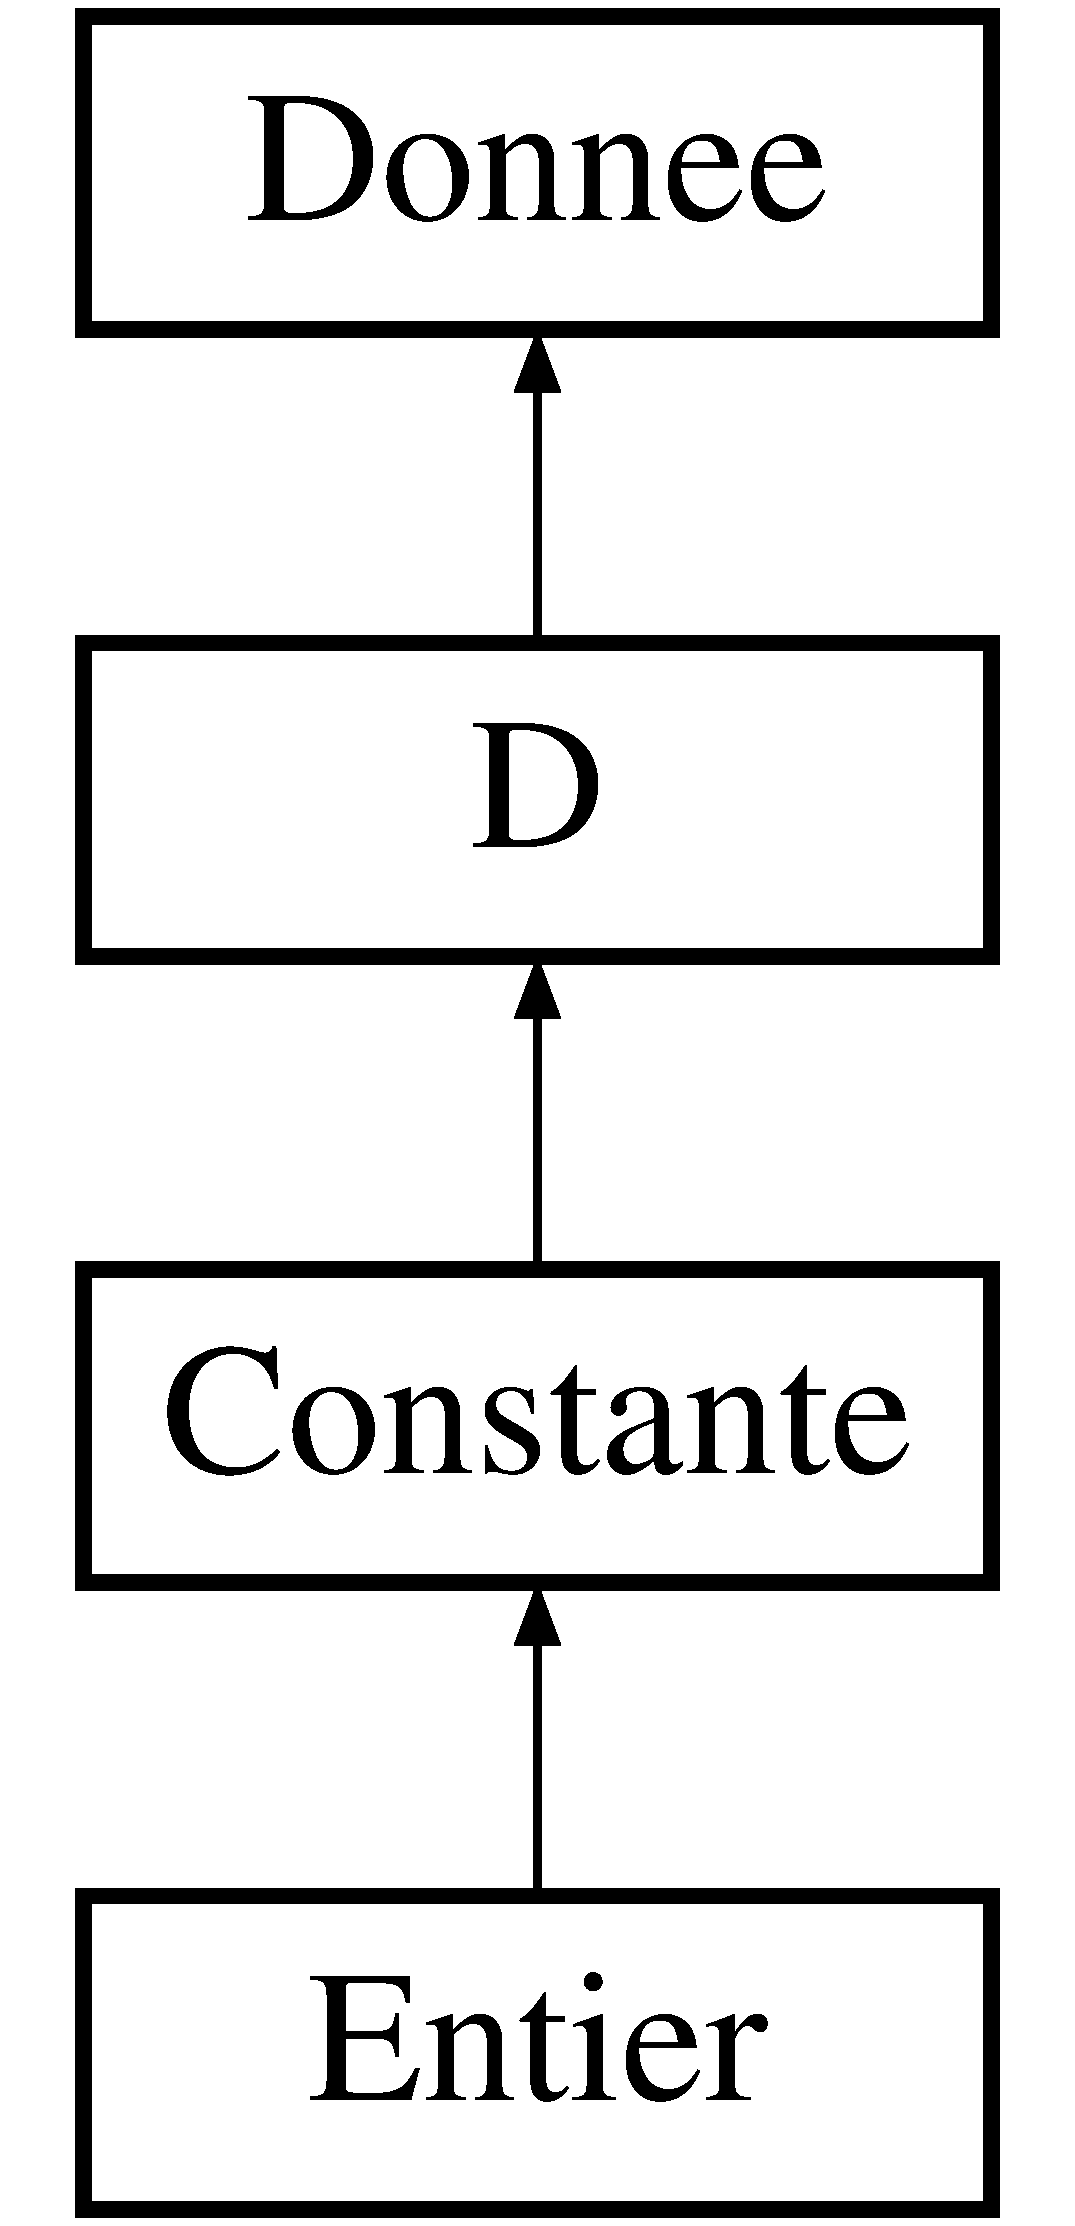
\includegraphics[height=4.000000cm]{class_entier}
\end{center}
\end{figure}
\subsection*{Fonctions membres publiques}
\begin{DoxyCompactItemize}
\item 
\hypertarget{class_entier_ab7343e7337fe0f74b26a370bd60e83fd}{{\bfseries Entier} (int val=0)}\label{class_entier_ab7343e7337fe0f74b26a370bd60e83fd}

\item 
\hypertarget{class_entier_afbd6f3cad81d75a4cb2fb142dcded828}{{\bfseries Entier} (const Q\-String \&s)}\label{class_entier_afbd6f3cad81d75a4cb2fb142dcded828}

\item 
\hypertarget{class_entier_a06090bab3375f1adba393192b7c87dec}{int {\bfseries get\-Data} ()}\label{class_entier_a06090bab3375f1adba393192b7c87dec}

\item 
\hypertarget{class_entier_ad70191b038f04dd46cf3c053d2b5428b}{\hyperlink{class_donnee}{Donnee} $\ast$ {\bfseries operator+} (\hyperlink{class_donnee}{Donnee} \&t)}\label{class_entier_ad70191b038f04dd46cf3c053d2b5428b}

\item 
\hypertarget{class_entier_a694ea4709a6e40c153069afb6b0bac33}{\hyperlink{class_donnee}{Donnee} $\ast$ {\bfseries operator/} (\hyperlink{class_donnee}{Donnee} \&t)}\label{class_entier_a694ea4709a6e40c153069afb6b0bac33}

\item 
\hypertarget{class_entier_a3ed8817d4078a4b792411bf0eb7642e7}{\hyperlink{class_donnee}{Donnee} $\ast$ {\bfseries operator$\ast$} (\hyperlink{class_donnee}{Donnee} \&t)}\label{class_entier_a3ed8817d4078a4b792411bf0eb7642e7}

\item 
\hypertarget{class_entier_a2f4322a6fbb75553b336521e492ee6ab}{\hyperlink{class_donnee}{Donnee} $\ast$ {\bfseries operator-\/} (\hyperlink{class_donnee}{Donnee} \&t)}\label{class_entier_a2f4322a6fbb75553b336521e492ee6ab}

\item 
\hypertarget{class_entier_a224f6a3c7982553c5e98870bb5ed2275}{\hyperlink{class_donnee}{Donnee} $\ast$ {\bfseries sinus} (bool degre=false)}\label{class_entier_a224f6a3c7982553c5e98870bb5ed2275}

\item 
\hypertarget{class_entier_a5931ccf5eb67467ab08148279f631aa5}{\hyperlink{class_donnee}{Donnee} $\ast$ {\bfseries pow} (\hyperlink{class_donnee}{Donnee} \&t)}\label{class_entier_a5931ccf5eb67467ab08148279f631aa5}

\item 
\hypertarget{class_entier_a101d8b37b994ba6b85d51106f212a973}{\hyperlink{class_donnee}{Donnee} $\ast$ {\bfseries mod} (\hyperlink{class_donnee}{Donnee} \&t)}\label{class_entier_a101d8b37b994ba6b85d51106f212a973}

\item 
\hypertarget{class_entier_a3f5445923ac6d5e820cf8fe5d2d4eec0}{\hyperlink{class_donnee}{Donnee} $\ast$ {\bfseries sign} ()}\label{class_entier_a3f5445923ac6d5e820cf8fe5d2d4eec0}

\item 
\hypertarget{class_entier_a830a88fb030f0920647e6fcd466df03c}{\hyperlink{class_donnee}{Donnee} $\ast$ {\bfseries cosinus} (bool degre=false)}\label{class_entier_a830a88fb030f0920647e6fcd466df03c}

\item 
\hypertarget{class_entier_ab47744f7e5b3d88bb605fc416eed17a9}{\hyperlink{class_donnee}{Donnee} $\ast$ {\bfseries tangente} (bool degre=false)}\label{class_entier_ab47744f7e5b3d88bb605fc416eed17a9}

\item 
\hypertarget{class_entier_a5a17040de5ebc53e066426be89915663}{\hyperlink{class_donnee}{Donnee} $\ast$ {\bfseries sinush} (bool degre=false)}\label{class_entier_a5a17040de5ebc53e066426be89915663}

\item 
\hypertarget{class_entier_a93a3cf4c1e434a1f51a332f28d7d4eac}{\hyperlink{class_donnee}{Donnee} $\ast$ {\bfseries cosinush} (bool degre=false)}\label{class_entier_a93a3cf4c1e434a1f51a332f28d7d4eac}

\item 
\hypertarget{class_entier_aaf0ca879f31b7385cf5f690bdea6647d}{\hyperlink{class_donnee}{Donnee} $\ast$ {\bfseries tangenteh} (bool degre=false)}\label{class_entier_aaf0ca879f31b7385cf5f690bdea6647d}

\item 
\hypertarget{class_entier_a03eddb6951874510d4682e71b1708f5d}{\hyperlink{class_donnee}{Donnee} $\ast$ {\bfseries ln} ()}\label{class_entier_a03eddb6951874510d4682e71b1708f5d}

\item 
\hypertarget{class_entier_afcbfd66b9411a464971d7269e824ed3b}{\hyperlink{class_donnee}{Donnee} $\ast$ {\bfseries log} ()}\label{class_entier_afcbfd66b9411a464971d7269e824ed3b}

\item 
\hypertarget{class_entier_a1a4ee280def58f34874e0b5307eb135e}{\hyperlink{class_donnee}{Donnee} $\ast$ {\bfseries inv} ()}\label{class_entier_a1a4ee280def58f34874e0b5307eb135e}

\item 
\hypertarget{class_entier_a207294a4cb8da36d6ea5ab61a9dd29a5}{\hyperlink{class_donnee}{Donnee} $\ast$ {\bfseries sqrt} ()}\label{class_entier_a207294a4cb8da36d6ea5ab61a9dd29a5}

\item 
\hypertarget{class_entier_af2206ecf5e7d67b3643e656df2a9734c}{\hyperlink{class_donnee}{Donnee} $\ast$ {\bfseries sqr} ()}\label{class_entier_af2206ecf5e7d67b3643e656df2a9734c}

\item 
\hypertarget{class_entier_ad5e0a60bba1c266338add6f367fbe667}{\hyperlink{class_donnee}{Donnee} $\ast$ {\bfseries cube} ()}\label{class_entier_ad5e0a60bba1c266338add6f367fbe667}

\item 
\hypertarget{class_entier_acb2b2a359d83307b67eb2ef3b5295c03}{\hyperlink{class_donnee}{Donnee} $\ast$ {\bfseries fact} ()}\label{class_entier_acb2b2a359d83307b67eb2ef3b5295c03}

\item 
\hypertarget{class_entier_ac9aab0cb446a34eb806b4c242c9216f2}{Q\-String {\bfseries to\-Q\-String} ()}\label{class_entier_ac9aab0cb446a34eb806b4c242c9216f2}

\end{DoxyCompactItemize}


La documentation de cette classe a été générée à partir des fichiers suivants \-:\begin{DoxyCompactItemize}
\item 
\hyperlink{_entier_8h}{Entier.\-h}\item 
entier.\-cpp\end{DoxyCompactItemize}

\hypertarget{class_expression}{\section{Référence de la classe Expression}
\label{class_expression}\index{Expression@{Expression}}
}
Graphe d'héritage de Expression\-:\begin{figure}[H]
\begin{center}
\leavevmode
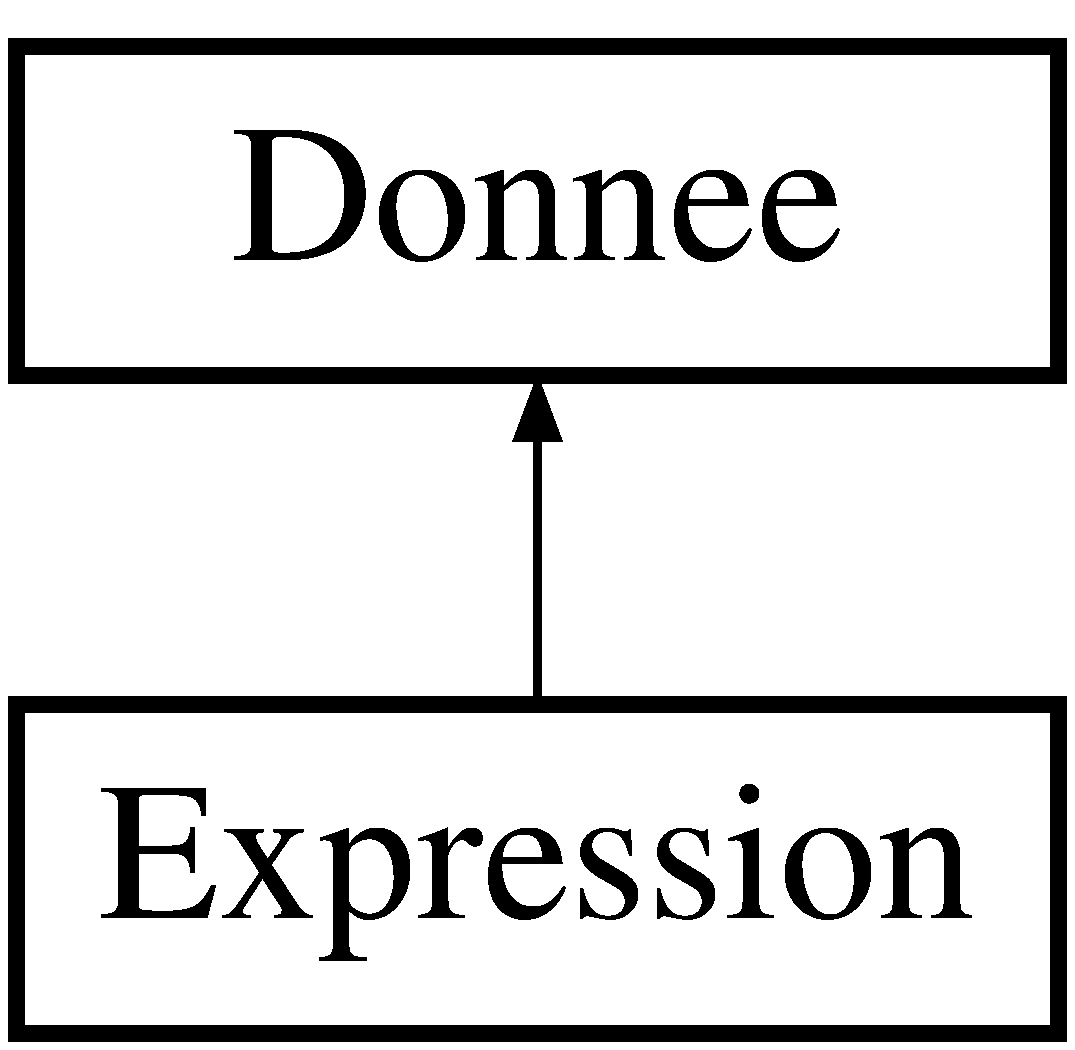
\includegraphics[height=2.000000cm]{class_expression}
\end{center}
\end{figure}
\subsection*{Fonctions membres publiques}
\begin{DoxyCompactItemize}
\item 
\hypertarget{class_expression_a2dfc0f1fe384a18adb7064f44aca0bed}{{\bfseries Expression} (Q\-String \&exp1)}\label{class_expression_a2dfc0f1fe384a18adb7064f44aca0bed}

\item 
\hypertarget{class_expression_aa7c32d233ec432effd8d9f7c8b592f2b}{\hyperlink{class_donnee}{Donnee} $\ast$ {\bfseries operator+} (\hyperlink{class_donnee}{Donnee} \&t)}\label{class_expression_aa7c32d233ec432effd8d9f7c8b592f2b}

\item 
\hypertarget{class_expression_a0f700db6943fe2ab9f5a9fc8c1d35243}{\hyperlink{class_donnee}{Donnee} $\ast$ {\bfseries operator/} (\hyperlink{class_donnee}{Donnee} \&t)}\label{class_expression_a0f700db6943fe2ab9f5a9fc8c1d35243}

\item 
\hypertarget{class_expression_a3bb3cc409248eaf44ad1d8bb41fb2b3f}{\hyperlink{class_donnee}{Donnee} $\ast$ {\bfseries operator$\ast$} (\hyperlink{class_donnee}{Donnee} \&t)}\label{class_expression_a3bb3cc409248eaf44ad1d8bb41fb2b3f}

\item 
\hypertarget{class_expression_a8d7bfb363774a0c68612ee42b3fff224}{\hyperlink{class_donnee}{Donnee} $\ast$ {\bfseries operator-\/} (\hyperlink{class_donnee}{Donnee} \&t)}\label{class_expression_a8d7bfb363774a0c68612ee42b3fff224}

\item 
\hypertarget{class_expression_a40d805e69e573bd135f750a10f083c6b}{\hyperlink{class_donnee}{Donnee} $\ast$ {\bfseries sinus} (bool degre=false)}\label{class_expression_a40d805e69e573bd135f750a10f083c6b}

\item 
\hypertarget{class_expression_a63cbf312c64ee81377f4cb43650fb619}{\hyperlink{class_donnee}{Donnee} $\ast$ {\bfseries pow} (\hyperlink{class_donnee}{Donnee} \&t)}\label{class_expression_a63cbf312c64ee81377f4cb43650fb619}

\item 
\hypertarget{class_expression_a35426bc4e0c8df5fff3aaeced4b0bff8}{\hyperlink{class_donnee}{Donnee} $\ast$ {\bfseries mod} (\hyperlink{class_donnee}{Donnee} \&t)}\label{class_expression_a35426bc4e0c8df5fff3aaeced4b0bff8}

\item 
\hypertarget{class_expression_a3e7568539e8938380421818c11fdb533}{\hyperlink{class_donnee}{Donnee} $\ast$ {\bfseries sign} ()}\label{class_expression_a3e7568539e8938380421818c11fdb533}

\item 
\hypertarget{class_expression_a34cc6843f0f96bf42e77f7de53eed85c}{\hyperlink{class_donnee}{Donnee} $\ast$ {\bfseries cosinus} (bool degre=false)}\label{class_expression_a34cc6843f0f96bf42e77f7de53eed85c}

\item 
\hypertarget{class_expression_a308ec79a0943a9cd11cf2ec1704ce8a5}{\hyperlink{class_donnee}{Donnee} $\ast$ {\bfseries tangente} (bool degre=false)}\label{class_expression_a308ec79a0943a9cd11cf2ec1704ce8a5}

\item 
\hypertarget{class_expression_a6d929568d5e9f4caa8c566a604f9184e}{\hyperlink{class_donnee}{Donnee} $\ast$ {\bfseries sinush} (bool degre=false)}\label{class_expression_a6d929568d5e9f4caa8c566a604f9184e}

\item 
\hypertarget{class_expression_ad88bc65b78d106b7d70c9311f5ba9c4b}{\hyperlink{class_donnee}{Donnee} $\ast$ {\bfseries cosinush} (bool degre=false)}\label{class_expression_ad88bc65b78d106b7d70c9311f5ba9c4b}

\item 
\hypertarget{class_expression_aeca12b23856e09f7df9bee6abef404fa}{\hyperlink{class_donnee}{Donnee} $\ast$ {\bfseries tangenteh} (bool degre=false)}\label{class_expression_aeca12b23856e09f7df9bee6abef404fa}

\item 
\hypertarget{class_expression_af43a59b7cf40046c1182657d30139418}{\hyperlink{class_donnee}{Donnee} $\ast$ {\bfseries ln} ()}\label{class_expression_af43a59b7cf40046c1182657d30139418}

\item 
\hypertarget{class_expression_adb5dc4e3d08d12f35fe2e128700e521a}{\hyperlink{class_donnee}{Donnee} $\ast$ {\bfseries log} ()}\label{class_expression_adb5dc4e3d08d12f35fe2e128700e521a}

\item 
\hypertarget{class_expression_a0323915714e5c8ce52a812a9a414f4a9}{\hyperlink{class_donnee}{Donnee} $\ast$ {\bfseries inv} ()}\label{class_expression_a0323915714e5c8ce52a812a9a414f4a9}

\item 
\hypertarget{class_expression_a283ae5ad2dc1ae7c5d8695d7eaca7f8c}{\hyperlink{class_donnee}{Donnee} $\ast$ {\bfseries sqrt} ()}\label{class_expression_a283ae5ad2dc1ae7c5d8695d7eaca7f8c}

\item 
\hypertarget{class_expression_af793a0f2ee48afb0e09e3e0bb3dffd6a}{\hyperlink{class_donnee}{Donnee} $\ast$ {\bfseries sqr} ()}\label{class_expression_af793a0f2ee48afb0e09e3e0bb3dffd6a}

\item 
\hypertarget{class_expression_a7fdb59a63420b5b056fd96e6d5e83fcb}{\hyperlink{class_donnee}{Donnee} $\ast$ {\bfseries cube} ()}\label{class_expression_a7fdb59a63420b5b056fd96e6d5e83fcb}

\item 
\hypertarget{class_expression_a7312cb958b6366f84fb4e01f58cd2119}{Q\-String {\bfseries eval} ()}\label{class_expression_a7312cb958b6366f84fb4e01f58cd2119}

\item 
\hypertarget{class_expression_a4404792ff4997e7c06a3242062825f5c}{Q\-String {\bfseries to\-Q\-String} ()}\label{class_expression_a4404792ff4997e7c06a3242062825f5c}

\end{DoxyCompactItemize}
\subsection*{Additional Inherited Members}


La documentation de cette classe a été générée à partir des fichiers suivants \-:\begin{DoxyCompactItemize}
\item 
\hyperlink{_expression_8h}{Expression.\-h}\item 
expression.\-cpp\end{DoxyCompactItemize}

\hypertarget{class_main_window}{\section{Référence de la classe Main\-Window}
\label{class_main_window}\index{Main\-Window@{Main\-Window}}
}
\subsection*{Signaux}
\begin{DoxyCompactItemize}
\item 
\hypertarget{class_main_window_a1e39eccc1e017799bda6b446b8280edf}{void {\bfseries push\-Stack\-\_\-signal} (const Q\-String \&)}\label{class_main_window_a1e39eccc1e017799bda6b446b8280edf}

\item 
\hypertarget{class_main_window_aed37073752de791b6ad06e41a8e9f1b2}{void {\bfseries clean\-List\-\_\-signal} ()}\label{class_main_window_aed37073752de791b6ad06e41a8e9f1b2}

\item 
\hypertarget{class_main_window_a94d40675237489fc9d25ccc868a4dcbd}{void {\bfseries refresh\-\_\-signal} ()}\label{class_main_window_a94d40675237489fc9d25ccc868a4dcbd}

\end{DoxyCompactItemize}
\subsection*{Fonctions membres publiques}
\begin{DoxyCompactItemize}
\item 
\hypertarget{class_main_window_ac8603055e732d11c01cfa8e44bff3ca2}{{\bfseries Main\-Window} (\hyperlink{class_pile}{Pile} \&pile, Q\-Widget $\ast$parent)}\label{class_main_window_ac8603055e732d11c01cfa8e44bff3ca2}

\end{DoxyCompactItemize}
\subsection*{Fonctions membres publiques statiques}
\begin{DoxyCompactItemize}
\item 
\hypertarget{class_main_window_a1dc154d1435cc7672dd35e82d3c466d4}{static \hyperlink{class_main_window}{Main\-Window} \& {\bfseries donne\-Instance} ()}\label{class_main_window_a1dc154d1435cc7672dd35e82d3c466d4}

\item 
\hypertarget{class_main_window_a67c2ee9b42435ed8bd98bcb194fc140d}{static void {\bfseries libere\-Instance} ()}\label{class_main_window_a67c2ee9b42435ed8bd98bcb194fc140d}

\end{DoxyCompactItemize}
\subsection*{Fonctions membres protégées}
\begin{DoxyCompactItemize}
\item 
\hypertarget{class_main_window_a6a060b895950b0ada1fc165f64288e14}{{\bfseries Main\-Window} (const \hyperlink{class_main_window}{Main\-Window} \&)}\label{class_main_window_a6a060b895950b0ada1fc165f64288e14}

\item 
\hypertarget{class_main_window_aa97903ff6a8044f898a59f243d3aa739}{void {\bfseries operator=} (const \hyperlink{class_main_window}{Main\-Window} \&)}\label{class_main_window_aa97903ff6a8044f898a59f243d3aa739}

\end{DoxyCompactItemize}


La documentation de cette classe a été générée à partir des fichiers suivants \-:\begin{DoxyCompactItemize}
\item 
\hyperlink{_main_window_8h}{Main\-Window.\-h}\item 
Main\-Window.\-cpp\end{DoxyCompactItemize}

\hypertarget{class_memento}{\section{Référence de la classe Memento}
\label{class_memento}\index{Memento@{Memento}}
}
\subsection*{Fonctions membres publiques}
\begin{DoxyCompactItemize}
\item 
\hypertarget{class_memento_a2db6a70bed1bedc3f5d93f8fa7d3a512}{\hyperlink{class_pile}{Pile} $\ast$ {\bfseries undo} ()}\label{class_memento_a2db6a70bed1bedc3f5d93f8fa7d3a512}

\item 
\hypertarget{class_memento_ab495f44281bd0060db9d8fe94306e99a}{\hyperlink{class_pile}{Pile} $\ast$ {\bfseries redo} ()}\label{class_memento_ab495f44281bd0060db9d8fe94306e99a}

\item 
\hypertarget{class_memento_a2e4928528bc1f886696ed5fb2524542a}{void {\bfseries add\-Memoire} (\hyperlink{class_pile}{Pile} $\ast$pile)}\label{class_memento_a2e4928528bc1f886696ed5fb2524542a}

\end{DoxyCompactItemize}


La documentation de cette classe a été générée à partir des fichiers suivants \-:\begin{DoxyCompactItemize}
\item 
\hyperlink{_memento_8h}{Memento.\-h}\item 
memento.\-cpp\end{DoxyCompactItemize}

\hypertarget{class_pile}{\section{Référence de la classe Pile}
\label{class_pile}\index{Pile@{Pile}}
}
\subsection*{Fonctions membres publiques}
\begin{DoxyCompactItemize}
\item 
\hypertarget{class_pile_ad65ece3020d11d8d58c2781150cdca44}{bool {\bfseries get\-Degre} () const }\label{class_pile_ad65ece3020d11d8d58c2781150cdca44}

\item 
\hypertarget{class_pile_abf4931bd506e4c892949c7b7b70fd097}{void {\bfseries set\-Degre} (bool deg)}\label{class_pile_abf4931bd506e4c892949c7b7b70fd097}

\item 
\hypertarget{class_pile_a555732cb1e82480697663ba299592d9d}{void {\bfseries sauvegarder} (Q\-String file\-Name)}\label{class_pile_a555732cb1e82480697663ba299592d9d}

\item 
\hypertarget{class_pile_a18026c4fab8cd91ddcec265c47039171}{void {\bfseries charger} (Q\-String file\-Name)}\label{class_pile_a18026c4fab8cd91ddcec265c47039171}

\item 
\hypertarget{class_pile_a13e1620ba0de2d1cd4b1f66f5356a8b4}{\hyperlink{class_pile}{Pile} \& {\bfseries clone} () const }\label{class_pile_a13e1620ba0de2d1cd4b1f66f5356a8b4}

\item 
\hypertarget{class_pile_aee5282e29d14470c8805b62830207306}{\hyperlink{class_pile}{Pile} \& {\bfseries duplique} () const }\label{class_pile_aee5282e29d14470c8805b62830207306}

\item 
\hypertarget{class_pile_a9105d1958c28860a1ed4b609c4701a41}{void {\bfseries set\-Memento} (\hyperlink{class_memento}{Memento} $\ast$\-\_\-g)}\label{class_pile_a9105d1958c28860a1ed4b609c4701a41}

\item 
\hypertarget{class_pile_a09fd751d9d6d0d3c861f97405756db56}{void {\bfseries set\-Nb\-Elt} (int nb)}\label{class_pile_a09fd751d9d6d0d3c861f97405756db56}

\item 
\hypertarget{class_pile_abf056806ae413b53d6ab9d6b7bbb6218}{\hyperlink{class_memento}{Memento} $\ast$ {\bfseries get\-Memento} () const }\label{class_pile_abf056806ae413b53d6ab9d6b7bbb6218}

\item 
\hypertarget{class_pile_ab6c3f9840427e2be87e0d76c8697fff5}{void {\bfseries swap} (unsigned int x, unsigned int y)}\label{class_pile_ab6c3f9840427e2be87e0d76c8697fff5}

\item 
\hypertarget{class_pile_ab2671569b6870d06fb94179e998e2e2e}{void {\bfseries sum} (const unsigned int x)}\label{class_pile_ab2671569b6870d06fb94179e998e2e2e}

\item 
\hypertarget{class_pile_a3993e0e33e78011663b15b9eb723d456}{void {\bfseries mean} (const unsigned int x)}\label{class_pile_a3993e0e33e78011663b15b9eb723d456}

\item 
\hypertarget{class_pile_a081f7843d01cae1f0f7be7d92e46d5d2}{void {\bfseries dup} ()}\label{class_pile_a081f7843d01cae1f0f7be7d92e46d5d2}

\item 
\hypertarget{class_pile_a7488ed257c6ceb16ed57a9fffb0726d5}{void {\bfseries drop} ()}\label{class_pile_a7488ed257c6ceb16ed57a9fffb0726d5}

\item 
\hypertarget{class_pile_a2f7afa189e97a23a836f07f9898538cf}{void {\bfseries addition} ()}\label{class_pile_a2f7afa189e97a23a836f07f9898538cf}

\item 
\hypertarget{class_pile_ab1827b113fff2c3fa59ebbe4c5902b1b}{void {\bfseries soustraction} ()}\label{class_pile_ab1827b113fff2c3fa59ebbe4c5902b1b}

\item 
\hypertarget{class_pile_a48ef99542609f5033f58ebd23189f698}{void {\bfseries division} ()}\label{class_pile_a48ef99542609f5033f58ebd23189f698}

\item 
\hypertarget{class_pile_ae5006ad08419fc6dcf65cbb4970199fe}{void {\bfseries multiplication} ()}\label{class_pile_ae5006ad08419fc6dcf65cbb4970199fe}

\item 
\hypertarget{class_pile_ac0be84cde5594e29678125e600bd8898}{void {\bfseries parser} (Q\-String s)}\label{class_pile_ac0be84cde5594e29678125e600bd8898}

\item 
\hypertarget{class_pile_acc36fadfcc65c9863a9d1d8d5dbe859a}{int {\bfseries get\-Nb} ()}\label{class_pile_acc36fadfcc65c9863a9d1d8d5dbe859a}

\item 
\hypertarget{class_pile_af91a4b277236024aa5aab9ef410881bb}{void {\bfseries undo} ()}\label{class_pile_af91a4b277236024aa5aab9ef410881bb}

\item 
\hypertarget{class_pile_aa8319a2921d86236d135cff700a5f833}{void {\bfseries redo} ()}\label{class_pile_aa8319a2921d86236d135cff700a5f833}

\item 
\hypertarget{class_pile_a20b1ece0cc61ecefc78e1a785ad8235f}{void {\bfseries pow} ()}\label{class_pile_a20b1ece0cc61ecefc78e1a785ad8235f}

\item 
\hypertarget{class_pile_a6d6092af4859ea5cefaa7959bb208774}{void {\bfseries mod} ()}\label{class_pile_a6d6092af4859ea5cefaa7959bb208774}

\item 
\hypertarget{class_pile_ad6ce16606725f1b2fa1028073afc3b75}{void {\bfseries sign} ()}\label{class_pile_ad6ce16606725f1b2fa1028073afc3b75}

\item 
\hypertarget{class_pile_a6d5405b44a45926264b48bd2df764798}{void {\bfseries sinus} (bool degre=false)}\label{class_pile_a6d5405b44a45926264b48bd2df764798}

\item 
\hypertarget{class_pile_a7962c91ddf8c1a453909150fb91608db}{void {\bfseries cosinus} (bool degre=false)}\label{class_pile_a7962c91ddf8c1a453909150fb91608db}

\item 
\hypertarget{class_pile_a45db8594e7934b5c9d749a9232afde4e}{void {\bfseries tangente} (bool degre=false)}\label{class_pile_a45db8594e7934b5c9d749a9232afde4e}

\item 
\hypertarget{class_pile_a4d12d390bd97a2432f41013ffc0dcc33}{void {\bfseries sinush} (bool degre=false)}\label{class_pile_a4d12d390bd97a2432f41013ffc0dcc33}

\item 
\hypertarget{class_pile_a44d3b913edb048c8d53d8f1f9549bfd3}{void {\bfseries cosinush} (bool degre=false)}\label{class_pile_a44d3b913edb048c8d53d8f1f9549bfd3}

\item 
\hypertarget{class_pile_a60cc5f271bbb70323af2aa0a40d40a3f}{void {\bfseries tangenteh} (bool degre=false)}\label{class_pile_a60cc5f271bbb70323af2aa0a40d40a3f}

\item 
\hypertarget{class_pile_ab22aed5e5178d32a3e47d8f4c599c9c4}{void {\bfseries ln} ()}\label{class_pile_ab22aed5e5178d32a3e47d8f4c599c9c4}

\item 
\hypertarget{class_pile_acaec5142e3afb5208091eecb6ac31f35}{void {\bfseries log} ()}\label{class_pile_acaec5142e3afb5208091eecb6ac31f35}

\item 
\hypertarget{class_pile_a040844b7b06a3aa8a25c47079858e5d4}{void {\bfseries inv} ()}\label{class_pile_a040844b7b06a3aa8a25c47079858e5d4}

\item 
\hypertarget{class_pile_a15e52c1dca0ef1e78af39c69f814e01a}{void {\bfseries sqrt} ()}\label{class_pile_a15e52c1dca0ef1e78af39c69f814e01a}

\item 
\hypertarget{class_pile_abd1c5a18cb8dd304e377d74fcec5a513}{void {\bfseries sqr} ()}\label{class_pile_abd1c5a18cb8dd304e377d74fcec5a513}

\item 
\hypertarget{class_pile_aee724c6620382459f78fab4fb08749eb}{void {\bfseries cube} ()}\label{class_pile_aee724c6620382459f78fab4fb08749eb}

\item 
\hypertarget{class_pile_a582a24a17a82fc63985900765b0499b4}{void {\bfseries fact} ()}\label{class_pile_a582a24a17a82fc63985900765b0499b4}

\item 
\hypertarget{class_pile_a9fbff00a90c14aca3b093b080c8b0f0b}{void {\bfseries eval} ()}\label{class_pile_a9fbff00a90c14aca3b093b080c8b0f0b}

\item 
\hypertarget{class_pile_adeeabcc051cf4a7449d117ff4a3a848a}{void {\bfseries set\-Type} (std\-::string d)}\label{class_pile_adeeabcc051cf4a7449d117ff4a3a848a}

\item 
\hypertarget{class_pile_a349a863ee08e9c966a9277cef6b55619}{std\-::string {\bfseries get\-Type} ()}\label{class_pile_a349a863ee08e9c966a9277cef6b55619}

\end{DoxyCompactItemize}


La documentation de cette classe a été générée à partir des fichiers suivants \-:\begin{DoxyCompactItemize}
\item 
\hyperlink{_pile_8h}{Pile.\-h}\item 
pile.\-cpp\end{DoxyCompactItemize}

\hypertarget{class_rationnel}{\section{Référence de la classe Rationnel}
\label{class_rationnel}\index{Rationnel@{Rationnel}}
}
Graphe d'héritage de Rationnel\-:\begin{figure}[H]
\begin{center}
\leavevmode
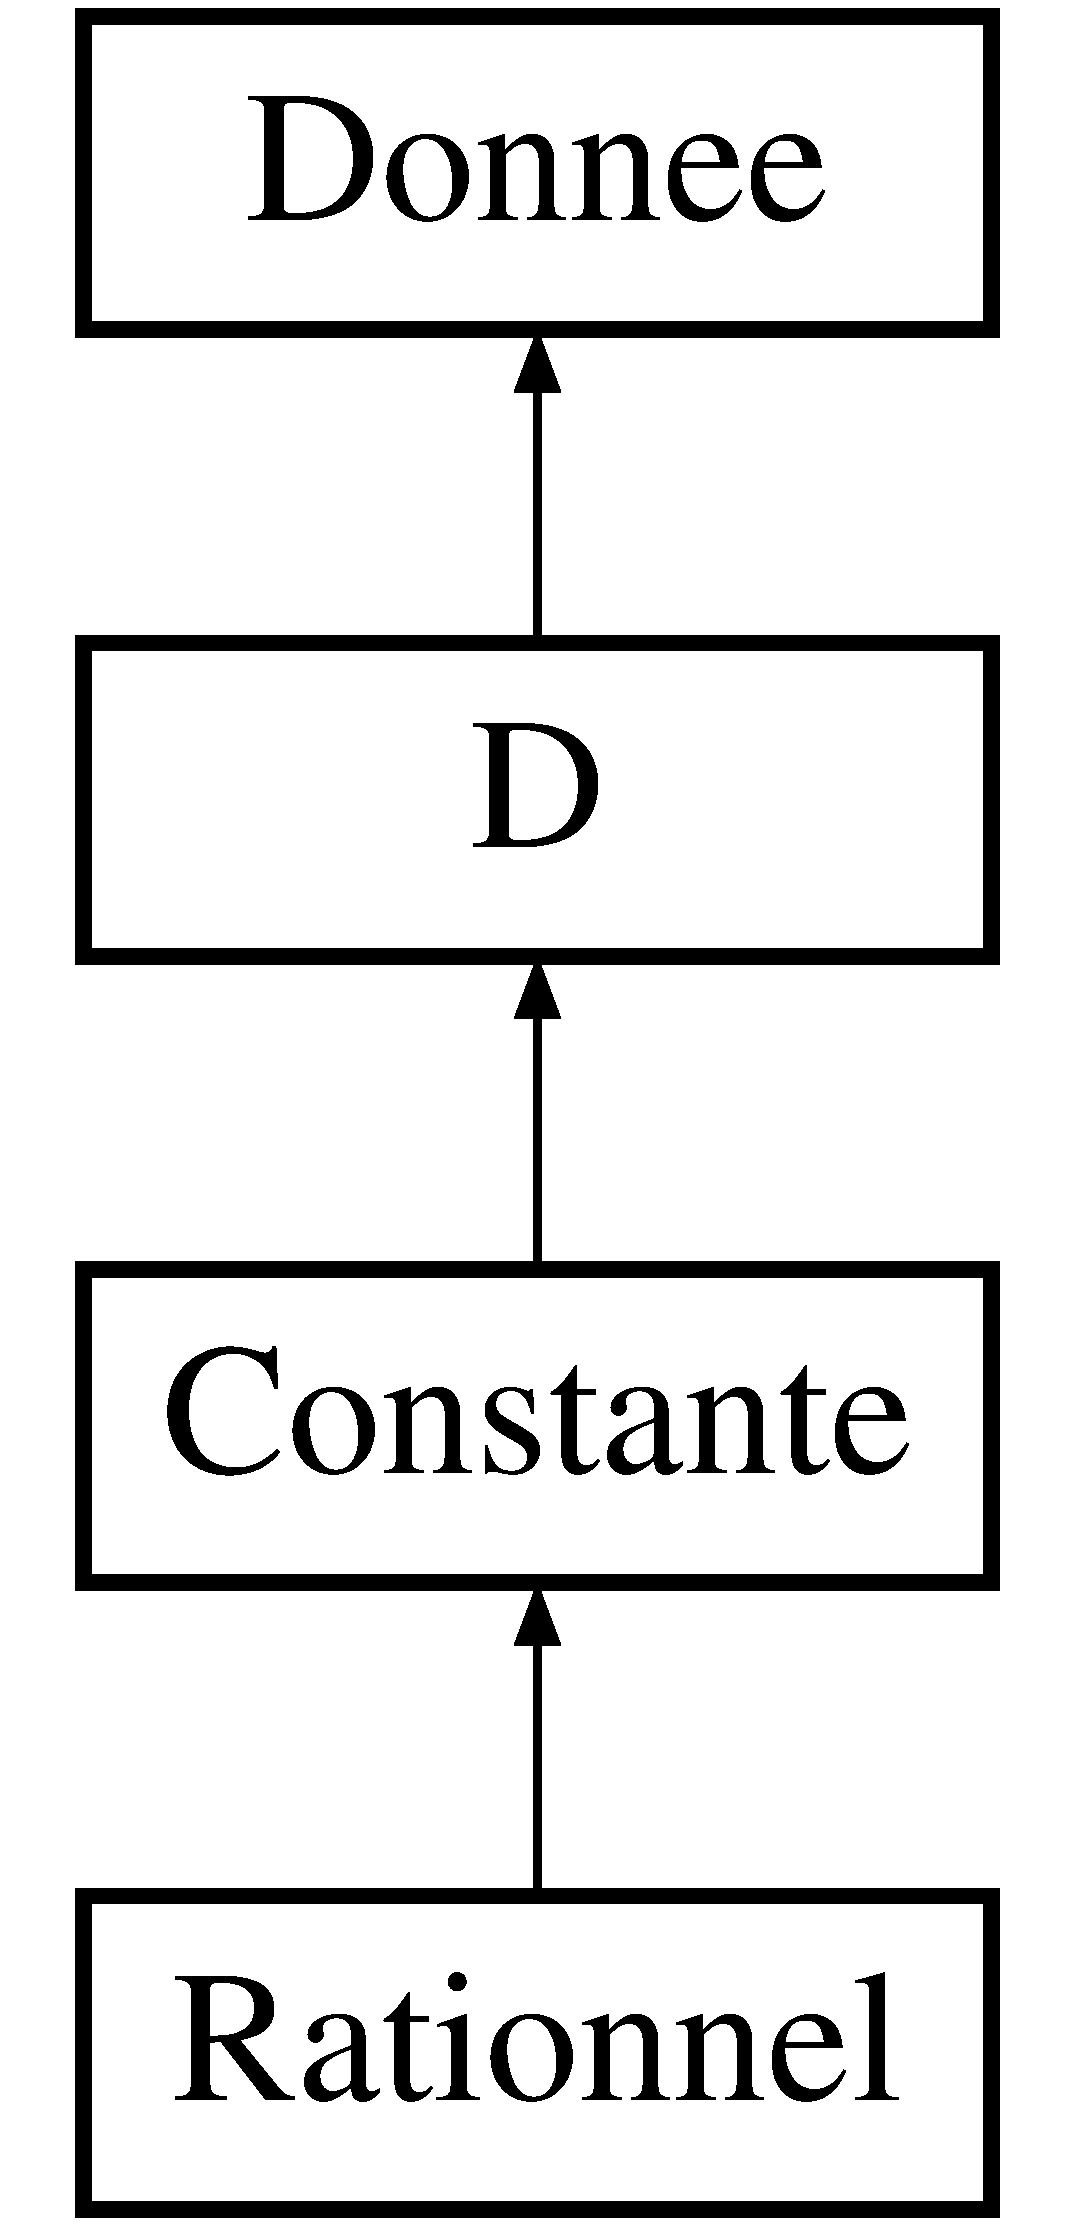
\includegraphics[height=4.000000cm]{class_rationnel}
\end{center}
\end{figure}
\subsection*{Fonctions membres publiques}
\begin{DoxyCompactItemize}
\item 
\hypertarget{class_rationnel_a455e4f7314244d5d81b83e55e16faed3}{{\bfseries Rationnel} (int \-\_\-num=0, int \-\_\-denum=1)}\label{class_rationnel_a455e4f7314244d5d81b83e55e16faed3}

\item 
\hypertarget{class_rationnel_a26a99758636a64b724fd6cf483695937}{{\bfseries Rationnel} (const Q\-String \&s)}\label{class_rationnel_a26a99758636a64b724fd6cf483695937}

\item 
\hypertarget{class_rationnel_aff1bffbfaa0f73c865c41abc03145d97}{\hyperlink{class_donnee}{Donnee} $\ast$ {\bfseries operator+} (\hyperlink{class_donnee}{Donnee} \&t)}\label{class_rationnel_aff1bffbfaa0f73c865c41abc03145d97}

\item 
\hypertarget{class_rationnel_a3996a46785798dfea002f21f2b7d6fea}{\hyperlink{class_donnee}{Donnee} $\ast$ {\bfseries operator/} (\hyperlink{class_donnee}{Donnee} \&t)}\label{class_rationnel_a3996a46785798dfea002f21f2b7d6fea}

\item 
\hypertarget{class_rationnel_acf49968b7a995107d29172e8fc1d81f6}{\hyperlink{class_donnee}{Donnee} $\ast$ {\bfseries operator$\ast$} (\hyperlink{class_donnee}{Donnee} \&t)}\label{class_rationnel_acf49968b7a995107d29172e8fc1d81f6}

\item 
\hypertarget{class_rationnel_afef41ceb9a7ac342623b10e51023fdf7}{\hyperlink{class_donnee}{Donnee} $\ast$ {\bfseries operator-\/} (\hyperlink{class_donnee}{Donnee} \&t)}\label{class_rationnel_afef41ceb9a7ac342623b10e51023fdf7}

\item 
\hypertarget{class_rationnel_a0b7a4036835138e1be1d57de8dfc7c75}{\hyperlink{class_donnee}{Donnee} $\ast$ {\bfseries sinus} (bool degre)}\label{class_rationnel_a0b7a4036835138e1be1d57de8dfc7c75}

\item 
\hypertarget{class_rationnel_a0c1d532ab3612bc69b00aa1bf94a3391}{\hyperlink{class_donnee}{Donnee} $\ast$ {\bfseries pow} (\hyperlink{class_donnee}{Donnee} \&t)}\label{class_rationnel_a0c1d532ab3612bc69b00aa1bf94a3391}

\item 
\hypertarget{class_rationnel_a9b98ddd641b5c3ba8aff3f26baf96e78}{\hyperlink{class_donnee}{Donnee} $\ast$ {\bfseries sign} ()}\label{class_rationnel_a9b98ddd641b5c3ba8aff3f26baf96e78}

\item 
\hypertarget{class_rationnel_a3be7da27abae6ea826c53d1659f7611e}{\hyperlink{class_donnee}{Donnee} $\ast$ {\bfseries cosinus} (bool degre)}\label{class_rationnel_a3be7da27abae6ea826c53d1659f7611e}

\item 
\hypertarget{class_rationnel_a0a67bd2a22d53299fcb2d402366ab9ab}{\hyperlink{class_donnee}{Donnee} $\ast$ {\bfseries tangente} (bool degre)}\label{class_rationnel_a0a67bd2a22d53299fcb2d402366ab9ab}

\item 
\hypertarget{class_rationnel_ae11232ca6d7d59b78e1d24949b9b6886}{\hyperlink{class_donnee}{Donnee} $\ast$ {\bfseries sinush} (bool degre)}\label{class_rationnel_ae11232ca6d7d59b78e1d24949b9b6886}

\item 
\hypertarget{class_rationnel_a49a356c69c7a422490adf46705d34d5b}{\hyperlink{class_donnee}{Donnee} $\ast$ {\bfseries cosinush} (bool degre)}\label{class_rationnel_a49a356c69c7a422490adf46705d34d5b}

\item 
\hypertarget{class_rationnel_af210c9838c41f2d8c09aea7dbf41fb13}{\hyperlink{class_donnee}{Donnee} $\ast$ {\bfseries tangenteh} (bool degre)}\label{class_rationnel_af210c9838c41f2d8c09aea7dbf41fb13}

\item 
\hypertarget{class_rationnel_abd8f38fb28b5ad1b763c4871d7ba7d55}{\hyperlink{class_donnee}{Donnee} $\ast$ {\bfseries ln} ()}\label{class_rationnel_abd8f38fb28b5ad1b763c4871d7ba7d55}

\item 
\hypertarget{class_rationnel_ac8db2758abad17b5d817349c5ae88fde}{\hyperlink{class_donnee}{Donnee} $\ast$ {\bfseries log} ()}\label{class_rationnel_ac8db2758abad17b5d817349c5ae88fde}

\item 
\hypertarget{class_rationnel_ab0098c07428153f4a7cad07ad89aa2bc}{\hyperlink{class_donnee}{Donnee} $\ast$ {\bfseries inv} ()}\label{class_rationnel_ab0098c07428153f4a7cad07ad89aa2bc}

\item 
\hypertarget{class_rationnel_a232edb3cbdfc4f2e91b73c5b78f719d1}{\hyperlink{class_donnee}{Donnee} $\ast$ {\bfseries sqrt} ()}\label{class_rationnel_a232edb3cbdfc4f2e91b73c5b78f719d1}

\item 
\hypertarget{class_rationnel_af5d7713691e8624a8ff81a34b2b9162e}{\hyperlink{class_donnee}{Donnee} $\ast$ {\bfseries sqr} ()}\label{class_rationnel_af5d7713691e8624a8ff81a34b2b9162e}

\item 
\hypertarget{class_rationnel_a8fef62cad68d2d4446f274d5caab5555}{\hyperlink{class_donnee}{Donnee} $\ast$ {\bfseries cube} ()}\label{class_rationnel_a8fef62cad68d2d4446f274d5caab5555}

\item 
\hypertarget{class_rationnel_a73ea78d08750aca3308f6cc3268925e0}{Q\-String {\bfseries to\-Q\-String} ()}\label{class_rationnel_a73ea78d08750aca3308f6cc3268925e0}

\item 
\hypertarget{class_rationnel_a731572a3c0fbfdaa57fc67725a87c219}{Q\-String {\bfseries eval} ()}\label{class_rationnel_a731572a3c0fbfdaa57fc67725a87c219}

\item 
\hypertarget{class_rationnel_ab01e543bba8ce3fb12a2dbb7a070b6e7}{void {\bfseries simplifie} ()}\label{class_rationnel_ab01e543bba8ce3fb12a2dbb7a070b6e7}

\item 
\hypertarget{class_rationnel_a30e5bf832f0cae6ce689edbdefda37a4}{int {\bfseries pgcd} (int, int) const }\label{class_rationnel_a30e5bf832f0cae6ce689edbdefda37a4}

\item 
\hypertarget{class_rationnel_a12fb184a604bd42e6d2bd5deda395812}{int {\bfseries get\-Num} ()}\label{class_rationnel_a12fb184a604bd42e6d2bd5deda395812}

\item 
\hypertarget{class_rationnel_ab7b58c2e2c2d305dbdf077b23d89b379}{int {\bfseries get\-Denum} ()}\label{class_rationnel_ab7b58c2e2c2d305dbdf077b23d89b379}

\end{DoxyCompactItemize}


La documentation de cette classe a été générée à partir des fichiers suivants \-:\begin{DoxyCompactItemize}
\item 
\hyperlink{_rationnel_8h}{Rationnel.\-h}\item 
rationnel.\-cpp\end{DoxyCompactItemize}

\hypertarget{class_reel}{\section{Référence de la classe Reel}
\label{class_reel}\index{Reel@{Reel}}
}
Graphe d'héritage de Reel\-:\begin{figure}[H]
\begin{center}
\leavevmode
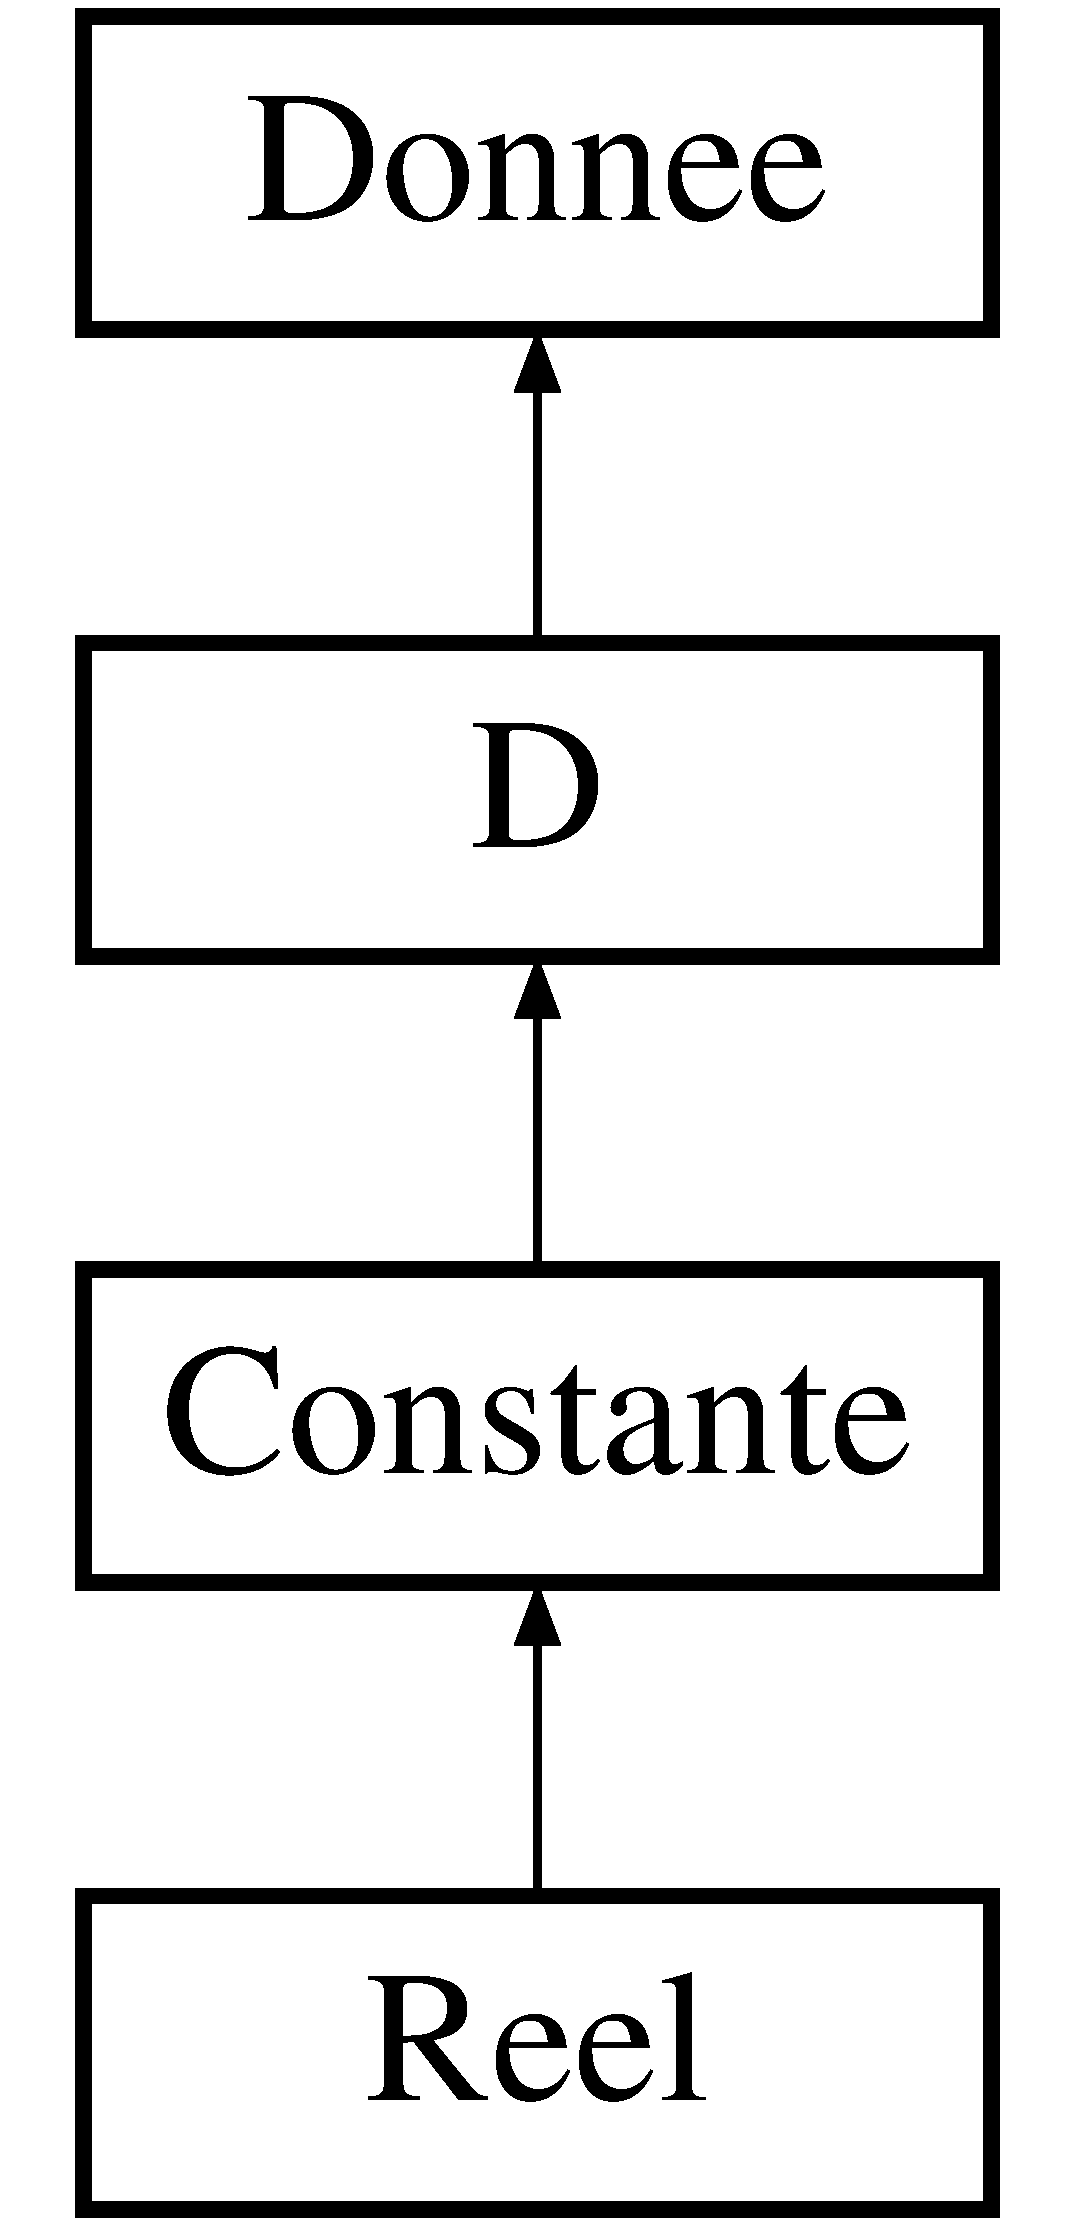
\includegraphics[height=4.000000cm]{class_reel}
\end{center}
\end{figure}
\subsection*{Fonctions membres publiques}
\begin{DoxyCompactItemize}
\item 
\hypertarget{class_reel_a10756227cbba51f1b70ad8ec1ac42f8b}{{\bfseries Reel} (double val=0)}\label{class_reel_a10756227cbba51f1b70ad8ec1ac42f8b}

\item 
\hypertarget{class_reel_aa44af559ad39232b46771a245e39172e}{{\bfseries Reel} (const Q\-String \&s)}\label{class_reel_aa44af559ad39232b46771a245e39172e}

\item 
\hypertarget{class_reel_a3965202bfe687a1f171c34cac92e1992}{double {\bfseries get\-Data} ()}\label{class_reel_a3965202bfe687a1f171c34cac92e1992}

\item 
\hypertarget{class_reel_a2bca56beb307d648f1d2a1acf2b832df}{\hyperlink{class_donnee}{Donnee} $\ast$ {\bfseries operator+} (\hyperlink{class_donnee}{Donnee} \&t)}\label{class_reel_a2bca56beb307d648f1d2a1acf2b832df}

\item 
\hypertarget{class_reel_acf3908140032378509352422477f3528}{\hyperlink{class_donnee}{Donnee} $\ast$ {\bfseries operator/} (\hyperlink{class_donnee}{Donnee} \&t)}\label{class_reel_acf3908140032378509352422477f3528}

\item 
\hypertarget{class_reel_a37ce50db66988d5922c93199ef625551}{\hyperlink{class_donnee}{Donnee} $\ast$ {\bfseries operator$\ast$} (\hyperlink{class_donnee}{Donnee} \&t)}\label{class_reel_a37ce50db66988d5922c93199ef625551}

\item 
\hypertarget{class_reel_afceac072f4568830292ae1ad6e5a17d0}{\hyperlink{class_donnee}{Donnee} $\ast$ {\bfseries operator-\/} (\hyperlink{class_donnee}{Donnee} \&t)}\label{class_reel_afceac072f4568830292ae1ad6e5a17d0}

\item 
\hypertarget{class_reel_adb33802e084c7a21ac42e98cf347a7e6}{\hyperlink{class_donnee}{Donnee} $\ast$ {\bfseries sinus} (bool degre)}\label{class_reel_adb33802e084c7a21ac42e98cf347a7e6}

\item 
\hypertarget{class_reel_ae07e77487c1223e485113e670a91be8b}{\hyperlink{class_donnee}{Donnee} $\ast$ {\bfseries pow} (\hyperlink{class_donnee}{Donnee} \&t)}\label{class_reel_ae07e77487c1223e485113e670a91be8b}

\item 
\hypertarget{class_reel_a418a1e0942783f9a538f53e2a6a855f6}{\hyperlink{class_donnee}{Donnee} $\ast$ {\bfseries sign} ()}\label{class_reel_a418a1e0942783f9a538f53e2a6a855f6}

\item 
\hypertarget{class_reel_a0b1ef439810d9d33b831d1a52550e97b}{\hyperlink{class_donnee}{Donnee} $\ast$ {\bfseries cosinus} (bool degre)}\label{class_reel_a0b1ef439810d9d33b831d1a52550e97b}

\item 
\hypertarget{class_reel_ab0a744004a6c92aef6a90d3e34645548}{\hyperlink{class_donnee}{Donnee} $\ast$ {\bfseries tangente} (bool degre)}\label{class_reel_ab0a744004a6c92aef6a90d3e34645548}

\item 
\hypertarget{class_reel_a20e43a4a8c7702a4a00eeb0cdb0e2cda}{\hyperlink{class_donnee}{Donnee} $\ast$ {\bfseries sinush} (bool degre)}\label{class_reel_a20e43a4a8c7702a4a00eeb0cdb0e2cda}

\item 
\hypertarget{class_reel_ad970a288a1a3b5c6695187c642069f62}{\hyperlink{class_donnee}{Donnee} $\ast$ {\bfseries cosinush} (bool degre)}\label{class_reel_ad970a288a1a3b5c6695187c642069f62}

\item 
\hypertarget{class_reel_a78414da3b388439db83ebcc41b7905c9}{\hyperlink{class_donnee}{Donnee} $\ast$ {\bfseries tangenteh} (bool degre)}\label{class_reel_a78414da3b388439db83ebcc41b7905c9}

\item 
\hypertarget{class_reel_ae1c0b2554cd9ea849fee4a1bacfb2114}{\hyperlink{class_donnee}{Donnee} $\ast$ {\bfseries ln} ()}\label{class_reel_ae1c0b2554cd9ea849fee4a1bacfb2114}

\item 
\hypertarget{class_reel_a098d92e2cee73718ae985101cb61de83}{\hyperlink{class_donnee}{Donnee} $\ast$ {\bfseries log} ()}\label{class_reel_a098d92e2cee73718ae985101cb61de83}

\item 
\hypertarget{class_reel_a53a64415bc8e47b712f40f445cc6f089}{\hyperlink{class_donnee}{Donnee} $\ast$ {\bfseries inv} ()}\label{class_reel_a53a64415bc8e47b712f40f445cc6f089}

\item 
\hypertarget{class_reel_a1ab432116e3316d4374cdb671c3f57c8}{\hyperlink{class_donnee}{Donnee} $\ast$ {\bfseries sqrt} ()}\label{class_reel_a1ab432116e3316d4374cdb671c3f57c8}

\item 
\hypertarget{class_reel_a0197e1162cc2db2bbfa745f268739f41}{\hyperlink{class_donnee}{Donnee} $\ast$ {\bfseries sqr} ()}\label{class_reel_a0197e1162cc2db2bbfa745f268739f41}

\item 
\hypertarget{class_reel_aa869cd43b6e40b0b8d0b51bfbe3114de}{\hyperlink{class_donnee}{Donnee} $\ast$ {\bfseries cube} ()}\label{class_reel_aa869cd43b6e40b0b8d0b51bfbe3114de}

\item 
\hypertarget{class_reel_ad71341b4e2aaa97cecb131412abaa8cf}{Q\-String {\bfseries to\-Q\-String} ()}\label{class_reel_ad71341b4e2aaa97cecb131412abaa8cf}

\item 
\hypertarget{class_reel_aab306676b02d5001b3bebe0b2e6468c4}{int {\bfseries get\-Decimales} ()}\label{class_reel_aab306676b02d5001b3bebe0b2e6468c4}

\end{DoxyCompactItemize}


La documentation de cette classe a été générée à partir des fichiers suivants \-:\begin{DoxyCompactItemize}
\item 
\hyperlink{_reel_8h}{Reel.\-h}\item 
reel.\-cpp\end{DoxyCompactItemize}

\chapter{Documentation des fichiers}
\hypertarget{_collection_pile_8h}{\section{Référence du fichier Collection\-Pile.\-h}
\label{_collection_pile_8h}\index{Collection\-Pile.\-h@{Collection\-Pile.\-h}}
}


\hyperlink{class_collection_pile}{Collection\-Pile} contient la classe \hyperlink{class_collection_pile}{Collection\-Pile} qui herite de vector et contient les piles pour ctrl + Z/ctrl + Y (undo/redo)  


{\ttfamily \#include $<$vector$>$}\\*
{\ttfamily \#include \char`\"{}Pile.\-h\char`\"{}}\\*
{\ttfamily \#include $<$Q\-String$>$}\\*
\subsection*{Classes}
\begin{DoxyCompactItemize}
\item 
class \hyperlink{class_collection_pile}{Collection\-Pile}
\end{DoxyCompactItemize}


\subsection{Description détaillée}
\hyperlink{class_collection_pile}{Collection\-Pile} contient la classe \hyperlink{class_collection_pile}{Collection\-Pile} qui herite de vector et contient les piles pour ctrl + Z/ctrl + Y (undo/redo) \begin{DoxyAuthor}{Auteur}
Cl�mence B\-L\-O\-T, Beno�t G\-A\-V\-A\-L\-D\-A 
\end{DoxyAuthor}

\hypertarget{_complexe_8h}{\section{Référence du fichier Complexe.\-h}
\label{_complexe_8h}\index{Complexe.\-h@{Complexe.\-h}}
}


\hyperlink{class_complexe}{Complexe} contient la classe complexe qui h�rite de \hyperlink{class_d}{D}, elle m�me h�ritant de Donn�e. cette classe sert � cr�er les objets complexes a\&b (lorsque le mode complexe est activ�)  


{\ttfamily \#include \char`\"{}Donnee.\-h\char`\"{}}\\*
{\ttfamily \#include $<$sstream$>$}\\*
{\ttfamily \#include $<$Q\-String$>$}\\*
{\ttfamily \#include \char`\"{}Constante.\-h\char`\"{}}\\*
{\ttfamily \#include \char`\"{}Donnee\-Factory.\-h\char`\"{}}\\*
{\ttfamily \#include \char`\"{}Reel.\-h\char`\"{}}\\*
{\ttfamily \#include \char`\"{}D.\-h\char`\"{}}\\*
\subsection*{Classes}
\begin{DoxyCompactItemize}
\item 
class \hyperlink{class_complexe}{Complexe}
\end{DoxyCompactItemize}


\subsection{Description détaillée}
\hyperlink{class_complexe}{Complexe} contient la classe complexe qui h�rite de \hyperlink{class_d}{D}, elle m�me h�ritant de Donn�e. cette classe sert � cr�er les objets complexes a\&b (lorsque le mode complexe est activ�) \begin{DoxyAuthor}{Auteur}
Cl�mence B\-L\-O\-T, Beno�t G\-A\-V\-A\-L\-D\-A 
\end{DoxyAuthor}

\begin{DoxyParams}{Paramètres}
{\em re} & partie r�elle \\
\hline
{\em im} & partie imaginaire \\
\hline
\end{DoxyParams}

\hypertarget{_constante_8h}{\section{Référence du fichier Constante.\-h}
\label{_constante_8h}\index{Constante.\-h@{Constante.\-h}}
}


\hyperlink{class_constante}{Constante} Class abstraite h�ritant de \hyperlink{class_d}{D} (qui h�rite de Donn�e) et engeandrant les classe \hyperlink{class_reel}{Reel}, \hyperlink{class_rationnel}{Rationnel}, \hyperlink{class_entier}{Entier}.  


{\ttfamily \#include \char`\"{}D.\-h\char`\"{}}\\*
{\ttfamily \#include \char`\"{}Donnee.\-h\char`\"{}}\\*
\subsection*{Classes}
\begin{DoxyCompactItemize}
\item 
class \hyperlink{class_constante}{Constante}
\end{DoxyCompactItemize}


\subsection{Description détaillée}
\hyperlink{class_constante}{Constante} Class abstraite h�ritant de \hyperlink{class_d}{D} (qui h�rite de Donn�e) et engeandrant les classe \hyperlink{class_reel}{Reel}, \hyperlink{class_rationnel}{Rationnel}, \hyperlink{class_entier}{Entier}. \begin{DoxyAuthor}{Auteur}
Cl�mence B\-L\-O\-T, Beno�t G\-A\-V\-A\-L\-D\-A 
\end{DoxyAuthor}

\hypertarget{_d_8h}{\section{Référence du fichier D.\-h}
\label{_d_8h}\index{D.\-h@{D.\-h}}
}


\hyperlink{class_d}{D} Classe h�ritant de \hyperlink{class_donnee}{Donnee} et engeandrant \hyperlink{class_complexe}{Complexe}.  


\subsection*{Classes}
\begin{DoxyCompactItemize}
\item 
class \hyperlink{class_d}{D}
\end{DoxyCompactItemize}


\subsection{Description détaillée}
\hyperlink{class_d}{D} Classe h�ritant de \hyperlink{class_donnee}{Donnee} et engeandrant \hyperlink{class_complexe}{Complexe}. \begin{DoxyAuthor}{Auteur}
Cl�mence B\-L\-O\-T, Beno�t G\-A\-V\-A\-L\-D\-A 
\end{DoxyAuthor}

\hypertarget{_dom_8h}{\section{Référence du fichier Dom.\-h}
\label{_dom_8h}\index{Dom.\-h@{Dom.\-h}}
}


\hyperlink{class_dom}{Dom} classe contenant les m�thodes d'�criture et de lecture de piles.  


{\ttfamily \#include $<$Q\-Text\-Stream$>$}\\*
{\ttfamily \#include $<$Qt\-Xml/\-Q\-Dom\-Document$>$}\\*
{\ttfamily \#include $<$Q\-File$>$}\\*
{\ttfamily \#include $<$Q\-Message\-Box$>$}\\*
{\ttfamily \#include $<$Q\-String$>$}\\*
{\ttfamily \#include \char`\"{}pile.\-h\char`\"{}}\\*
\subsection*{Classes}
\begin{DoxyCompactItemize}
\item 
class \hyperlink{class_dom}{Dom}
\end{DoxyCompactItemize}


\subsection{Description détaillée}
\hyperlink{class_dom}{Dom} classe contenant les m�thodes d'�criture et de lecture de piles. \begin{DoxyAuthor}{Auteur}
Cl�mence B\-L\-O\-T, Beno�t G\-A\-V\-A\-L\-D\-A 
\end{DoxyAuthor}

\hypertarget{_donnee_8h}{\section{Référence du fichier Donnee.\-h}
\label{_donnee_8h}\index{Donnee.\-h@{Donnee.\-h}}
}


Donne contient la classe abstraite qui chapeaute les classes des diff�rents types de donn�es.  


{\ttfamily \#include $<$sstream$>$}\\*
{\ttfamily \#include $<$Q\-String$>$}\\*
{\ttfamily \#include $<$Q\-Text\-Stream$>$}\\*
{\ttfamily \#include \char`\"{}Donnee\-Exception.\-h\char`\"{}}\\*
{\ttfamily \#include $<$Q\-Message\-Box$>$}\\*
\subsection*{Classes}
\begin{DoxyCompactItemize}
\item 
class \hyperlink{class_donnee}{Donnee}
\end{DoxyCompactItemize}
\subsection*{Variables}
\begin{DoxyCompactItemize}
\item 
\hypertarget{_donnee_8h_a9fb8a895035d83abe9846f2a33470060}{const float {\bfseries M\-\_\-\-P\-I} = 3.\-14159}\label{_donnee_8h_a9fb8a895035d83abe9846f2a33470060}

\end{DoxyCompactItemize}


\subsection{Description détaillée}
Donne contient la classe abstraite qui chapeaute les classes des diff�rents types de donn�es. \begin{DoxyAuthor}{Auteur}
Cl�mence B\-L\-O\-T, Beno�t G\-A\-V\-A\-L\-D\-A 
\end{DoxyAuthor}

\hypertarget{_donnee_exception_8h}{\section{Référence du fichier Donnee\-Exception.\-h}
\label{_donnee_exception_8h}\index{Donnee\-Exception.\-h@{Donnee\-Exception.\-h}}
}


Donne\-Exception classe qui g�re les exceptions.  


{\ttfamily \#include $<$stdexcept$>$}\\*
{\ttfamily \#include $<$string$>$}\\*
{\ttfamily \#include $<$Q\-String$>$}\\*
\subsection*{Classes}
\begin{DoxyCompactItemize}
\item 
class \hyperlink{class_donnee_exception}{Donnee\-Exception}
\end{DoxyCompactItemize}


\subsection{Description détaillée}
Donne\-Exception classe qui g�re les exceptions. \begin{DoxyAuthor}{Auteur}
Cl�mence B\-L\-O\-T, Beno�t G\-A\-V\-A\-L\-D\-A 
\end{DoxyAuthor}

\begin{DoxyParams}{Paramètres}
{\em info} & string qui contient les informations sur l'erreur \\
\hline
\end{DoxyParams}

\hypertarget{_donnee_factory_8h}{\section{Référence du fichier Donnee\-Factory.\-h}
\label{_donnee_factory_8h}\index{Donnee\-Factory.\-h@{Donnee\-Factory.\-h}}
}


Donne\-Factory Classe � instance unique qui cr�er les Objets de type \hyperlink{class_donnee}{Donnee} (\hyperlink{class_reel}{Reel}, \hyperlink{class_rationnel}{Rationnel}, \hyperlink{class_entier}{Entier}, \hyperlink{class_complexe}{Complexe})  


{\ttfamily \#include $<$Q\-String$>$}\\*
{\ttfamily \#include \char`\"{}Donnee.\-h\char`\"{}}\\*
{\ttfamily \#include $<$Q\-String\-List$>$}\\*
\subsection*{Classes}
\begin{DoxyCompactItemize}
\item 
class \hyperlink{class_donnee_factory}{Donnee\-Factory}
\end{DoxyCompactItemize}


\subsection{Description détaillée}
Donne\-Factory Classe � instance unique qui cr�er les Objets de type \hyperlink{class_donnee}{Donnee} (\hyperlink{class_reel}{Reel}, \hyperlink{class_rationnel}{Rationnel}, \hyperlink{class_entier}{Entier}, \hyperlink{class_complexe}{Complexe}) \begin{DoxyAuthor}{Auteur}
Cl�mence B\-L\-O\-T, Beno�t G\-A\-V\-A\-L\-D\-A 
\end{DoxyAuthor}

\begin{DoxyParams}{Paramètres}
{\em instance} & Instance unique \\
\hline
\end{DoxyParams}

\hypertarget{_entier_8h}{\section{Référence du fichier Entier.\-h}
\label{_entier_8h}\index{Entier.\-h@{Entier.\-h}}
}


\hyperlink{class_entier}{Entier} contient la classe permet de g�n�rer les objets stockant les entiers.  


{\ttfamily \#include \char`\"{}Donnee.\-h\char`\"{}}\\*
{\ttfamily \#include $<$sstream$>$}\\*
{\ttfamily \#include $<$Q\-String$>$}\\*
{\ttfamily \#include \char`\"{}Constante.\-h\char`\"{}}\\*
{\ttfamily \#include $<$Q\-Reg\-Exp$>$}\\*
\subsection*{Classes}
\begin{DoxyCompactItemize}
\item 
class \hyperlink{class_entier}{Entier}
\end{DoxyCompactItemize}


\subsection{Description détaillée}
\hyperlink{class_entier}{Entier} contient la classe permet de g�n�rer les objets stockant les entiers. \begin{DoxyAuthor}{Auteur}
Cl�mence B\-L\-O\-T, Beno�t G\-A\-V\-A\-L\-D\-A 
\end{DoxyAuthor}

\begin{DoxyParams}{Paramètres}
{\em data} & La donn�e � stocker \\
\hline
\end{DoxyParams}

\hypertarget{_expression_8h}{\section{Référence du fichier Expression.\-h}
\label{_expression_8h}\index{Expression.\-h@{Expression.\-h}}
}


\hyperlink{class_expression}{Expression} contient la classe permet de g�n�rer les objets stockant les expressions.  


{\ttfamily \#include $<$Q\-String$>$}\\*
{\ttfamily \#include \char`\"{}Donnee.\-h\char`\"{}}\\*
\subsection*{Classes}
\begin{DoxyCompactItemize}
\item 
class \hyperlink{class_expression}{Expression}
\end{DoxyCompactItemize}


\subsection{Description détaillée}
\hyperlink{class_expression}{Expression} contient la classe permet de g�n�rer les objets stockant les expressions. \begin{DoxyAuthor}{Auteur}
Cl�mence B\-L\-O\-T, Beno�t G\-A\-V\-A\-L\-D\-A 
\end{DoxyAuthor}

\begin{DoxyParams}{Paramètres}
{\em exp} & \hyperlink{class_expression}{Expression} � stocker \\
\hline
\end{DoxyParams}

\hypertarget{_main_window_8h}{\section{Référence du fichier Main\-Window.\-h}
\label{_main_window_8h}\index{Main\-Window.\-h@{Main\-Window.\-h}}
}


\hyperlink{class_main_window}{Main\-Window} Classe de l'affichage de la fen�tre principale.  


{\ttfamily \#include $<$Q\-Main\-Window$>$}\\*
{\ttfamily \#include $<$Q\-Stack$>$}\\*
{\ttfamily \#include \char`\"{}Pile.\-h\char`\"{}}\\*
{\ttfamily \#include \char`\"{}Donnee.\-h\char`\"{}}\\*
{\ttfamily \#include $<$Q\-String$>$}\\*
{\ttfamily \#include \char`\"{}Collection\-Pile.\-h\char`\"{}}\\*
{\ttfamily \#include $<$Q\-File\-Dialog$>$}\\*
{\ttfamily \#include $<$Q\-Message\-Box$>$}\\*
\subsection*{Classes}
\begin{DoxyCompactItemize}
\item 
class \hyperlink{class_main_window}{Main\-Window}
\end{DoxyCompactItemize}


\subsection{Description détaillée}
\hyperlink{class_main_window}{Main\-Window} Classe de l'affichage de la fen�tre principale. \begin{DoxyAuthor}{Auteur}
Cl�mence B\-L\-O\-T, Beno�t G\-A\-V\-A\-L\-D\-A 
\end{DoxyAuthor}

\hypertarget{_memento_8h}{\section{Référence du fichier Memento.\-h}
\label{_memento_8h}\index{Memento.\-h@{Memento.\-h}}
}


\hyperlink{class_memento}{Memento} Comprend les m�thodes n�cessaire � la r�alisation de undo/redo.  


{\ttfamily \#include $<$Q\-Vector$>$}\\*
{\ttfamily \#include $<$Q\-Stack$>$}\\*
{\ttfamily \#include \char`\"{}Donnee.\-h\char`\"{}}\\*
\subsection*{Classes}
\begin{DoxyCompactItemize}
\item 
class \hyperlink{class_memento}{Memento}
\end{DoxyCompactItemize}


\subsection{Description détaillée}
\hyperlink{class_memento}{Memento} Comprend les m�thodes n�cessaire � la r�alisation de undo/redo. \begin{DoxyAuthor}{Auteur}
Cl�mence B\-L\-O\-T, Beno�t G\-A\-V\-A\-L\-D\-A 
\end{DoxyAuthor}

\begin{DoxyParams}{Paramètres}
{\em current\-Stack} & \hyperlink{class_pile}{Pile} courante \\
\hline
{\em tab\-Pile} & tableau de pile de type Q\-Vector qui permet de garder en m�moire les pr�c�dentes piles. \\
\hline
\end{DoxyParams}

\hypertarget{_pile_8h}{\section{Référence du fichier Pile.\-h}
\label{_pile_8h}\index{Pile.\-h@{Pile.\-h}}
}


\hyperlink{class_pile}{Pile} Classe de nos piles, h�ritant de Q\-Stack. Ce sont des piles de \hyperlink{class_donnee}{Donnee}.  


{\ttfamily \#include $<$Q\-Stack$>$}\\*
{\ttfamily \#include \char`\"{}Donnee.\-h\char`\"{}}\\*
{\ttfamily \#include $<$Q\-String$>$}\\*
{\ttfamily \#include $<$sstream$>$}\\*
{\ttfamily \#include $<$Q\-String\-List$>$}\\*
{\ttfamily \#include \char`\"{}Donnee\-Factory.\-h\char`\"{}}\\*
{\ttfamily \#include \char`\"{}Memento.\-h\char`\"{}}\\*
\subsection*{Classes}
\begin{DoxyCompactItemize}
\item 
class \hyperlink{class_pile}{Pile}
\end{DoxyCompactItemize}


\subsection{Description détaillée}
\hyperlink{class_pile}{Pile} Classe de nos piles, h�ritant de Q\-Stack. Ce sont des piles de \hyperlink{class_donnee}{Donnee}. \begin{DoxyAuthor}{Auteur}
Cl�mence B\-L\-O\-T, Beno�t G\-A\-V\-A\-L\-D\-A 
\end{DoxyAuthor}

\begin{DoxyParams}{Paramètres}
{\em nb\-Elt} & Nombre d'�l�ment de la pile \\
\hline
{\em g} & \hyperlink{class_memento}{Memento} qui permet le undo redo \\
\hline
{\em degree} & bol�en qui est vrai si on est en mode degr�, faux si en radian. \\
\hline
{\em type} & string\{\hyperlink{class_complexe}{Complexe}, \hyperlink{class_reel}{Reel}, \hyperlink{class_rationnel}{Rationnel}, \hyperlink{class_entier}{Entier}\} qui indique le mode de la calculatrice. \\
\hline
\end{DoxyParams}

\hypertarget{_rationnel_8h}{\section{Référence du fichier Rationnel.\-h}
\label{_rationnel_8h}\index{Rationnel.\-h@{Rationnel.\-h}}
}


\hyperlink{class_rationnel}{Rationnel} contient la classe permet de g�n�rer les objets stockant les rationnels.  


{\ttfamily \#include \char`\"{}Donnee.\-h\char`\"{}}\\*
{\ttfamily \#include $<$iostream$>$}\\*
{\ttfamily \#include $<$sstream$>$}\\*
{\ttfamily \#include $<$Q\-String$>$}\\*
{\ttfamily \#include \char`\"{}Constante.\-h\char`\"{}}\\*
{\ttfamily \#include \char`\"{}Donnee\-Exception.\-h\char`\"{}}\\*
{\ttfamily \#include $<$Q\-Reg\-Exp$>$}\\*
\subsection*{Classes}
\begin{DoxyCompactItemize}
\item 
class \hyperlink{class_rationnel}{Rationnel}
\end{DoxyCompactItemize}


\subsection{Description détaillée}
\hyperlink{class_rationnel}{Rationnel} contient la classe permet de g�n�rer les objets stockant les rationnels. \begin{DoxyAuthor}{Auteur}
Cl�mence B\-L\-O\-T, Beno�t G\-A\-V\-A\-L\-D\-A 
\end{DoxyAuthor}

\begin{DoxyParams}{Paramètres}
{\em num} & num�rateur \\
\hline
{\em denum} & d�nominateur \\
\hline
\end{DoxyParams}

\hypertarget{_reel_8h}{\section{Référence du fichier Reel.\-h}
\label{_reel_8h}\index{Reel.\-h@{Reel.\-h}}
}


\hyperlink{class_reel}{Reel} contient la classe permet de g�n�rer les objets stockant les r�els.  


{\ttfamily \#include \char`\"{}Donnee.\-h\char`\"{}}\\*
{\ttfamily \#include $<$sstream$>$}\\*
{\ttfamily \#include $<$Q\-String$>$}\\*
{\ttfamily \#include \char`\"{}Constante.\-h\char`\"{}}\\*
{\ttfamily \#include $<$Q\-Reg\-Exp$>$}\\*
\subsection*{Classes}
\begin{DoxyCompactItemize}
\item 
class \hyperlink{class_reel}{Reel}
\end{DoxyCompactItemize}


\subsection{Description détaillée}
\hyperlink{class_reel}{Reel} contient la classe permet de g�n�rer les objets stockant les r�els. \begin{DoxyAuthor}{Auteur}
Cl�mence B\-L\-O\-T, Beno�t G\-A\-V\-A\-L\-D\-A 
\end{DoxyAuthor}

\begin{DoxyParams}{Paramètres}
{\em data} & r�el � stocker \\
\hline
\end{DoxyParams}

\printindex
\end{document}
